\documentclass[12pt]{article}
\textwidth 6.5in \oddsidemargin .06in \evensidemargin .06in
\textheight 8.5in \topmargin -.6in
\newtheorem{remark}{Remark}[section]
\newtheorem{Lemma}{Lemma}[section]
\newtheorem{Corollary}{Corollary}[section]
\newtheorem{Theorem}{Theorem}[section]
\newtheorem{Proposition}{Proposition}[section]
\newtheorem{Definition}{Defintion}[section]
\newtheorem{Example}{Example}[section] 
\renewcommand{\theequation}{\arabic{section}.\arabic{equation}}

\linespread{1.5}
\usepackage{amsmath}
\usepackage{amsfonts}
\usepackage[breakable]{tcolorbox}
%\usepackage{parskip} 
\usepackage{ctex}
\usepackage{graphicx}

\let\Oldincludegraphics\includegraphics
    % Ensure that by default, figures have no caption (until we provide a
    % proper Figure object with a Caption API and a way to capture that
    % in the conversion process - todo).
\usepackage{caption}
%\DeclareCaptionFormat{nocaption}{}
%\captionsetup{format=nocaption,aboveskip=0pt,belowskip=0pt}

%\usepackage{float}
%\floatplacement{figure}{H} % forces figures to be placed at the correct location
\usepackage{xcolor} % Allow colors to be defined
\usepackage{enumerate} % Needed for markdown enumerations to work
\usepackage{geometry} % Used to adjust the document margins
\usepackage{amsmath} % Equations
\usepackage{amssymb} % Equations
\usepackage{textcomp} % defines textquotesingle
    % Hack from http://tex.stackexchange.com/a/47451/13684:
\AtBeginDocument{%
\def\PYZsq{\textquotesingle}% Upright quotes in Pygmentized code
    }
\usepackage{upquote} % Upright quotes for verbatim code
\usepackage{eurosym} % defines \euro

\usepackage{iftex}
\ifPDFTeX
\usepackage[T1]{fontenc}
\IfFileExists{alphabeta.sty}{
              \usepackage{alphabeta}
          }{
              \usepackage[mathletters]{ucs}
              \usepackage[utf8x]{inputenc}
          }
    \else
        \usepackage{fontspec}
        \usepackage{unicode-math}
    \fi

    \usepackage{fancyvrb} % verbatim replacement that allows latex
    \usepackage{grffile} % extends the file name processing of package graphics 
                         % to support a larger range
    \makeatletter % fix for old versions of grffile with XeLaTeX
    \@ifpackagelater{grffile}{2019/11/01}
    {
      % Do nothing on new versions
    }
    {
      \def\Gread@@xetex#1{%
        \IfFileExists{"\Gin@base".bb}%
        {\Gread@eps{\Gin@base.bb}}%
        {\Gread@@xetex@aux#1}%
      }
    }
    \makeatother
    \usepackage[Export]{adjustbox} % Used to constrain images to a maximum size
    \adjustboxset{max size={0.9\linewidth}{0.9\paperheight}}

    % The hyperref package gives us a pdf with properly built
    % internal navigation ('pdf bookmarks' for the table of contents,
    % internal cross-reference links, web links for URLs, etc.)
    \usepackage{hyperref}
    % The default LaTeX title has an obnoxious amount of whitespace. By default,
    % titling removes some of it. It also provides customization options.
    \usepackage{titling}
    \usepackage{longtable} % longtable support required by pandoc >1.10
    \usepackage{booktabs}  % table support for pandoc > 1.12.2
    \usepackage{array}     % table support for pandoc >= 2.11.3
    \usepackage{calc}      % table minipage width calculation for pandoc >= 2.11.1
    \usepackage[inline]{enumitem} % IRkernel/repr support (it uses the enumerate* environment)
    \usepackage[normalem]{ulem} % ulem is needed to support strikethroughs (\sout)
                                % normalem makes italics be italics, not underlines
    \usepackage{mathrsfs}
    

    
    % Colors for the hyperref package
    \definecolor{urlcolor}{rgb}{0,.145,.698}
    \definecolor{linkcolor}{rgb}{.71,0.21,0.01}
    \definecolor{citecolor}{rgb}{.12,.54,.11}

    % ANSI colors
    \definecolor{ansi-black}{HTML}{3E424D}
    \definecolor{ansi-black-intense}{HTML}{282C36}
    \definecolor{ansi-red}{HTML}{E75C58}
    \definecolor{ansi-red-intense}{HTML}{B22B31}
    \definecolor{ansi-green}{HTML}{00A250}
    \definecolor{ansi-green-intense}{HTML}{007427}
    \definecolor{ansi-yellow}{HTML}{DDB62B}
    \definecolor{ansi-yellow-intense}{HTML}{B27D12}
    \definecolor{ansi-blue}{HTML}{208FFB}
    \definecolor{ansi-blue-intense}{HTML}{0065CA}
    \definecolor{ansi-magenta}{HTML}{D160C4}
    \definecolor{ansi-magenta-intense}{HTML}{A03196}
    \definecolor{ansi-cyan}{HTML}{60C6C8}
    \definecolor{ansi-cyan-intense}{HTML}{258F8F}
    \definecolor{ansi-white}{HTML}{C5C1B4}
    \definecolor{ansi-white-intense}{HTML}{A1A6B2}
    \definecolor{ansi-default-inverse-fg}{HTML}{FFFFFF}
    \definecolor{ansi-default-inverse-bg}{HTML}{000000}

    % common color for the border for error outputs.
    \definecolor{outerrorbackground}{HTML}{FFDFDF}

    % commands and environments needed by pandoc snippets
    % extracted from the output of `pandoc -s`
    \providecommand{\tightlist}{%
      \setlength{\itemsep}{0pt}\setlength{\parskip}{0pt}}
    \DefineVerbatimEnvironment{Highlighting}{Verbatim}{commandchars=\\\{\}}
    % Add ',fontsize=\small' for more characters per line
    \newenvironment{Shaded}{}{}
    \newcommand{\KeywordTok}[1]{\textcolor[rgb]{0.00,0.44,0.13}{\textbf{{#1}}}}
    \newcommand{\DataTypeTok}[1]{\textcolor[rgb]{0.56,0.13,0.00}{{#1}}}
    \newcommand{\DecValTok}[1]{\textcolor[rgb]{0.25,0.63,0.44}{{#1}}}
    \newcommand{\BaseNTok}[1]{\textcolor[rgb]{0.25,0.63,0.44}{{#1}}}
    \newcommand{\FloatTok}[1]{\textcolor[rgb]{0.25,0.63,0.44}{{#1}}}
    \newcommand{\CharTok}[1]{\textcolor[rgb]{0.25,0.44,0.63}{{#1}}}
    \newcommand{\StringTok}[1]{\textcolor[rgb]{0.25,0.44,0.63}{{#1}}}
    \newcommand{\CommentTok}[1]{\textcolor[rgb]{0.38,0.63,0.69}{\textit{{#1}}}}
    \newcommand{\OtherTok}[1]{\textcolor[rgb]{0.00,0.44,0.13}{{#1}}}
    \newcommand{\AlertTok}[1]{\textcolor[rgb]{1.00,0.00,0.00}{\textbf{{#1}}}}
    \newcommand{\FunctionTok}[1]{\textcolor[rgb]{0.02,0.16,0.49}{{#1}}}
    \newcommand{\RegionMarkerTok}[1]{{#1}}
    \newcommand{\ErrorTok}[1]{\textcolor[rgb]{1.00,0.00,0.00}{\textbf{{#1}}}}
    \newcommand{\NormalTok}[1]{{#1}}
    
    % Additional commands for more recent versions of Pandoc
    \newcommand{\ConstantTok}[1]{\textcolor[rgb]{0.53,0.00,0.00}{{#1}}}
    \newcommand{\SpecialCharTok}[1]{\textcolor[rgb]{0.25,0.44,0.63}{{#1}}}
    \newcommand{\VerbatimStringTok}[1]{\textcolor[rgb]{0.25,0.44,0.63}{{#1}}}
    \newcommand{\SpecialStringTok}[1]{\textcolor[rgb]{0.73,0.40,0.53}{{#1}}}
    \newcommand{\ImportTok}[1]{{#1}}
    \newcommand{\DocumentationTok}[1]{\textcolor[rgb]{0.73,0.13,0.13}{\textit{{#1}}}}
    \newcommand{\AnnotationTok}[1]{\textcolor[rgb]{0.38,0.63,0.69}{\textbf{\textit{{#1}}}}}
    \newcommand{\CommentVarTok}[1]{\textcolor[rgb]{0.38,0.63,0.69}{\textbf{\textit{{#1}}}}}
    \newcommand{\VariableTok}[1]{\textcolor[rgb]{0.10,0.09,0.49}{{#1}}}
    \newcommand{\ControlFlowTok}[1]{\textcolor[rgb]{0.00,0.44,0.13}{\textbf{{#1}}}}
    \newcommand{\OperatorTok}[1]{\textcolor[rgb]{0.40,0.40,0.40}{{#1}}}
    \newcommand{\BuiltInTok}[1]{{#1}}
    \newcommand{\ExtensionTok}[1]{{#1}}
    \newcommand{\PreprocessorTok}[1]{\textcolor[rgb]{0.74,0.48,0.00}{{#1}}}
    \newcommand{\AttributeTok}[1]{\textcolor[rgb]{0.49,0.56,0.16}{{#1}}}
    \newcommand{\InformationTok}[1]{\textcolor[rgb]{0.38,0.63,0.69}{\textbf{\textit{{#1}}}}}
    \newcommand{\WarningTok}[1]{\textcolor[rgb]{0.38,0.63,0.69}{\textbf{\textit{{#1}}}}}
    
    
    % Define a nice break command that doesn't care if a line doesn't already
    % exist.
    \def\br{\hspace*{\fill} \\* }
    % Math Jax compatibility definitions
    \def\gt{>}
    \def\lt{<}
    \let\Oldtex\TeX
    \let\Oldlatex\LaTeX
    \renewcommand{\TeX}{\textrm{\Oldtex}}
    \renewcommand{\LaTeX}{\textrm{\Oldlatex}}
    % Document parameters
    % Document title
    \title{Untitled}
    
    
    
    
    
% Pygments definitions
\makeatletter
\def\PY@reset{\let\PY@it=\relax \let\PY@bf=\relax%
    \let\PY@ul=\relax \let\PY@tc=\relax%
    \let\PY@bc=\relax \let\PY@ff=\relax}
\def\PY@tok#1{\csname PY@tok@#1\endcsname}
\def\PY@toks#1+{\ifx\relax#1\empty\else%
    \PY@tok{#1}\expandafter\PY@toks\fi}
\def\PY@do#1{\PY@bc{\PY@tc{\PY@ul{%
    \PY@it{\PY@bf{\PY@ff{#1}}}}}}}
\def\PY#1#2{\PY@reset\PY@toks#1+\relax+\PY@do{#2}}

\@namedef{PY@tok@w}{\def\PY@tc##1{\textcolor[rgb]{0.73,0.73,0.73}{##1}}}
\@namedef{PY@tok@c}{\let\PY@it=\textit\def\PY@tc##1{\textcolor[rgb]{0.24,0.48,0.48}{##1}}}
\@namedef{PY@tok@cp}{\def\PY@tc##1{\textcolor[rgb]{0.61,0.40,0.00}{##1}}}
\@namedef{PY@tok@k}{\let\PY@bf=\textbf\def\PY@tc##1{\textcolor[rgb]{0.00,0.50,0.00}{##1}}}
\@namedef{PY@tok@kp}{\def\PY@tc##1{\textcolor[rgb]{0.00,0.50,0.00}{##1}}}
\@namedef{PY@tok@kt}{\def\PY@tc##1{\textcolor[rgb]{0.69,0.00,0.25}{##1}}}
\@namedef{PY@tok@o}{\def\PY@tc##1{\textcolor[rgb]{0.40,0.40,0.40}{##1}}}
\@namedef{PY@tok@ow}{\let\PY@bf=\textbf\def\PY@tc##1{\textcolor[rgb]{0.67,0.13,1.00}{##1}}}
\@namedef{PY@tok@nb}{\def\PY@tc##1{\textcolor[rgb]{0.00,0.50,0.00}{##1}}}
\@namedef{PY@tok@nf}{\def\PY@tc##1{\textcolor[rgb]{0.00,0.00,1.00}{##1}}}
\@namedef{PY@tok@nc}{\let\PY@bf=\textbf\def\PY@tc##1{\textcolor[rgb]{0.00,0.00,1.00}{##1}}}
\@namedef{PY@tok@nn}{\let\PY@bf=\textbf\def\PY@tc##1{\textcolor[rgb]{0.00,0.00,1.00}{##1}}}
\@namedef{PY@tok@ne}{\let\PY@bf=\textbf\def\PY@tc##1{\textcolor[rgb]{0.80,0.25,0.22}{##1}}}
\@namedef{PY@tok@nv}{\def\PY@tc##1{\textcolor[rgb]{0.10,0.09,0.49}{##1}}}
\@namedef{PY@tok@no}{\def\PY@tc##1{\textcolor[rgb]{0.53,0.00,0.00}{##1}}}
\@namedef{PY@tok@nl}{\def\PY@tc##1{\textcolor[rgb]{0.46,0.46,0.00}{##1}}}
\@namedef{PY@tok@ni}{\let\PY@bf=\textbf\def\PY@tc##1{\textcolor[rgb]{0.44,0.44,0.44}{##1}}}
\@namedef{PY@tok@na}{\def\PY@tc##1{\textcolor[rgb]{0.41,0.47,0.13}{##1}}}
\@namedef{PY@tok@nt}{\let\PY@bf=\textbf\def\PY@tc##1{\textcolor[rgb]{0.00,0.50,0.00}{##1}}}
\@namedef{PY@tok@nd}{\def\PY@tc##1{\textcolor[rgb]{0.67,0.13,1.00}{##1}}}
\@namedef{PY@tok@s}{\def\PY@tc##1{\textcolor[rgb]{0.73,0.13,0.13}{##1}}}
\@namedef{PY@tok@sd}{\let\PY@it=\textit\def\PY@tc##1{\textcolor[rgb]{0.73,0.13,0.13}{##1}}}
\@namedef{PY@tok@si}{\let\PY@bf=\textbf\def\PY@tc##1{\textcolor[rgb]{0.64,0.35,0.47}{##1}}}
\@namedef{PY@tok@se}{\let\PY@bf=\textbf\def\PY@tc##1{\textcolor[rgb]{0.67,0.36,0.12}{##1}}}
\@namedef{PY@tok@sr}{\def\PY@tc##1{\textcolor[rgb]{0.64,0.35,0.47}{##1}}}
\@namedef{PY@tok@ss}{\def\PY@tc##1{\textcolor[rgb]{0.10,0.09,0.49}{##1}}}
\@namedef{PY@tok@sx}{\def\PY@tc##1{\textcolor[rgb]{0.00,0.50,0.00}{##1}}}
\@namedef{PY@tok@m}{\def\PY@tc##1{\textcolor[rgb]{0.40,0.40,0.40}{##1}}}
\@namedef{PY@tok@gh}{\let\PY@bf=\textbf\def\PY@tc##1{\textcolor[rgb]{0.00,0.00,0.50}{##1}}}
\@namedef{PY@tok@gu}{\let\PY@bf=\textbf\def\PY@tc##1{\textcolor[rgb]{0.50,0.00,0.50}{##1}}}
\@namedef{PY@tok@gd}{\def\PY@tc##1{\textcolor[rgb]{0.63,0.00,0.00}{##1}}}
\@namedef{PY@tok@gi}{\def\PY@tc##1{\textcolor[rgb]{0.00,0.52,0.00}{##1}}}
\@namedef{PY@tok@gr}{\def\PY@tc##1{\textcolor[rgb]{0.89,0.00,0.00}{##1}}}
\@namedef{PY@tok@ge}{\let\PY@it=\textit}
\@namedef{PY@tok@gs}{\let\PY@bf=\textbf}
\@namedef{PY@tok@gp}{\let\PY@bf=\textbf\def\PY@tc##1{\textcolor[rgb]{0.00,0.00,0.50}{##1}}}
\@namedef{PY@tok@go}{\def\PY@tc##1{\textcolor[rgb]{0.44,0.44,0.44}{##1}}}
\@namedef{PY@tok@gt}{\def\PY@tc##1{\textcolor[rgb]{0.00,0.27,0.87}{##1}}}
\@namedef{PY@tok@err}{\def\PY@bc##1{{\setlength{\fboxsep}{\string -\fboxrule}\fcolorbox[rgb]{1.00,0.00,0.00}{1,1,1}{\strut ##1}}}}
\@namedef{PY@tok@kc}{\let\PY@bf=\textbf\def\PY@tc##1{\textcolor[rgb]{0.00,0.50,0.00}{##1}}}
\@namedef{PY@tok@kd}{\let\PY@bf=\textbf\def\PY@tc##1{\textcolor[rgb]{0.00,0.50,0.00}{##1}}}
\@namedef{PY@tok@kn}{\let\PY@bf=\textbf\def\PY@tc##1{\textcolor[rgb]{0.00,0.50,0.00}{##1}}}
\@namedef{PY@tok@kr}{\let\PY@bf=\textbf\def\PY@tc##1{\textcolor[rgb]{0.00,0.50,0.00}{##1}}}
\@namedef{PY@tok@bp}{\def\PY@tc##1{\textcolor[rgb]{0.00,0.50,0.00}{##1}}}
\@namedef{PY@tok@fm}{\def\PY@tc##1{\textcolor[rgb]{0.00,0.00,1.00}{##1}}}
\@namedef{PY@tok@vc}{\def\PY@tc##1{\textcolor[rgb]{0.10,0.09,0.49}{##1}}}
\@namedef{PY@tok@vg}{\def\PY@tc##1{\textcolor[rgb]{0.10,0.09,0.49}{##1}}}
\@namedef{PY@tok@vi}{\def\PY@tc##1{\textcolor[rgb]{0.10,0.09,0.49}{##1}}}
\@namedef{PY@tok@vm}{\def\PY@tc##1{\textcolor[rgb]{0.10,0.09,0.49}{##1}}}
\@namedef{PY@tok@sa}{\def\PY@tc##1{\textcolor[rgb]{0.73,0.13,0.13}{##1}}}
\@namedef{PY@tok@sb}{\def\PY@tc##1{\textcolor[rgb]{0.73,0.13,0.13}{##1}}}
\@namedef{PY@tok@sc}{\def\PY@tc##1{\textcolor[rgb]{0.73,0.13,0.13}{##1}}}
\@namedef{PY@tok@dl}{\def\PY@tc##1{\textcolor[rgb]{0.73,0.13,0.13}{##1}}}
\@namedef{PY@tok@s2}{\def\PY@tc##1{\textcolor[rgb]{0.73,0.13,0.13}{##1}}}
\@namedef{PY@tok@sh}{\def\PY@tc##1{\textcolor[rgb]{0.73,0.13,0.13}{##1}}}
\@namedef{PY@tok@s1}{\def\PY@tc##1{\textcolor[rgb]{0.73,0.13,0.13}{##1}}}
\@namedef{PY@tok@mb}{\def\PY@tc##1{\textcolor[rgb]{0.40,0.40,0.40}{##1}}}
\@namedef{PY@tok@mf}{\def\PY@tc##1{\textcolor[rgb]{0.40,0.40,0.40}{##1}}}
\@namedef{PY@tok@mh}{\def\PY@tc##1{\textcolor[rgb]{0.40,0.40,0.40}{##1}}}
\@namedef{PY@tok@mi}{\def\PY@tc##1{\textcolor[rgb]{0.40,0.40,0.40}{##1}}}
\@namedef{PY@tok@il}{\def\PY@tc##1{\textcolor[rgb]{0.40,0.40,0.40}{##1}}}
\@namedef{PY@tok@mo}{\def\PY@tc##1{\textcolor[rgb]{0.40,0.40,0.40}{##1}}}
\@namedef{PY@tok@ch}{\let\PY@it=\textit\def\PY@tc##1{\textcolor[rgb]{0.24,0.48,0.48}{##1}}}
\@namedef{PY@tok@cm}{\let\PY@it=\textit\def\PY@tc##1{\textcolor[rgb]{0.24,0.48,0.48}{##1}}}
\@namedef{PY@tok@cpf}{\let\PY@it=\textit\def\PY@tc##1{\textcolor[rgb]{0.24,0.48,0.48}{##1}}}
\@namedef{PY@tok@c1}{\let\PY@it=\textit\def\PY@tc##1{\textcolor[rgb]{0.24,0.48,0.48}{##1}}}
\@namedef{PY@tok@cs}{\let\PY@it=\textit\def\PY@tc##1{\textcolor[rgb]{0.24,0.48,0.48}{##1}}}

\def\PYZbs{\char`\\}
\def\PYZus{\char`\_}
\def\PYZob{\char`\{}
\def\PYZcb{\char`\}}
\def\PYZca{\char`\^}
\def\PYZam{\char`\&}
\def\PYZlt{\char`\<}
\def\PYZgt{\char`\>}
\def\PYZsh{\char`\#}
\def\PYZpc{\char`\%}
\def\PYZdl{\char`\$}
\def\PYZhy{\char`\-}
\def\PYZsq{\char`\'}
\def\PYZdq{\char`\"}
\def\PYZti{\char`\~}
% for compatibility with earlier versions
\def\PYZat{@}
\def\PYZlb{[}
\def\PYZrb{]}
\makeatother


    % For linebreaks inside Verbatim environment from package fancyvrb. 
    \makeatletter
        \newbox\Wrappedcontinuationbox 
        \newbox\Wrappedvisiblespacebox 
        \newcommand*\Wrappedvisiblespace {\textcolor{red}{\textvisiblespace}} 
        \newcommand*\Wrappedcontinuationsymbol {\textcolor{red}{\llap{\tiny$\m@th\hookrightarrow$}}} 
        \newcommand*\Wrappedcontinuationindent {3ex } 
        \newcommand*\Wrappedafterbreak {\kern\Wrappedcontinuationindent\copy\Wrappedcontinuationbox} 
        \newcommand*\Wrappedbreaksatspecials {% 
            \def\PYGZus{\discretionary{\char`\_}{\Wrappedafterbreak}{\char`\_}}% 
            \def\PYGZob{\discretionary{}{\Wrappedafterbreak\char`\{}{\char`\{}}% 
            \def\PYGZcb{\discretionary{\char`\}}{\Wrappedafterbreak}{\char`\}}}% 
            \def\PYGZca{\discretionary{\char`\^}{\Wrappedafterbreak}{\char`\^}}% 
            \def\PYGZam{\discretionary{\char`\&}{\Wrappedafterbreak}{\char`\&}}% 
            \def\PYGZlt{\discretionary{}{\Wrappedafterbreak\char`\<}{\char`\<}}% 
            \def\PYGZgt{\discretionary{\char`\>}{\Wrappedafterbreak}{\char`\>}}% 
            \def\PYGZsh{\discretionary{}{\Wrappedafterbreak\char`\#}{\char`\#}}% 
            \def\PYGZpc{\discretionary{}{\Wrappedafterbreak\char`\%}{\char`\%}}% 
            \def\PYGZdl{\discretionary{}{\Wrappedafterbreak\char`\$}{\char`\$}}% 
            \def\PYGZhy{\discretionary{\char`\-}{\Wrappedafterbreak}{\char`\-}}% 
            \def\PYGZsq{\discretionary{}{\Wrappedafterbreak\textquotesingle}{\textquotesingle}}% 
            \def\PYGZdq{\discretionary{}{\Wrappedafterbreak\char`\"}{\char`\"}}% 
            \def\PYGZti{\discretionary{\char`\~}{\Wrappedafterbreak}{\char`\~}}% 
        } 
        % Some characters . , ; ? ! / are not pygmentized. 
        % This macro makes them "active" and they will insert potential linebreaks 
        \newcommand*\Wrappedbreaksatpunct {% 
            \lccode`\~`\.\lowercase{\def~}{\discretionary{\hbox{\char`\.}}{\Wrappedafterbreak}{\hbox{\char`\.}}}% 
            \lccode`\~`\,\lowercase{\def~}{\discretionary{\hbox{\char`\,}}{\Wrappedafterbreak}{\hbox{\char`\,}}}% 
            \lccode`\~`\;\lowercase{\def~}{\discretionary{\hbox{\char`\;}}{\Wrappedafterbreak}{\hbox{\char`\;}}}% 
            \lccode`\~`\:\lowercase{\def~}{\discretionary{\hbox{\char`\:}}{\Wrappedafterbreak}{\hbox{\char`\:}}}% 
            \lccode`\~`\?\lowercase{\def~}{\discretionary{\hbox{\char`\?}}{\Wrappedafterbreak}{\hbox{\char`\?}}}% 
            \lccode`\~`\!\lowercase{\def~}{\discretionary{\hbox{\char`\!}}{\Wrappedafterbreak}{\hbox{\char`\!}}}% 
            \lccode`\~`\/\lowercase{\def~}{\discretionary{\hbox{\char`\/}}{\Wrappedafterbreak}{\hbox{\char`\/}}}% 
            \catcode`\.\active
            \catcode`\,\active 
            \catcode`\;\active
            \catcode`\:\active
            \catcode`\?\active
            \catcode`\!\active
            \catcode`\/\active 
            \lccode`\~`\~ 	
        }
    \makeatother

    \let\OriginalVerbatim=\Verbatim
    \makeatletter
    \renewcommand{\Verbatim}[1][1]{%
        %\parskip\z@skip
        \sbox\Wrappedcontinuationbox {\Wrappedcontinuationsymbol}%
        \sbox\Wrappedvisiblespacebox {\FV@SetupFont\Wrappedvisiblespace}%
        \def\FancyVerbFormatLine ##1{\hsize\linewidth
            \vtop{\raggedright\hyphenpenalty\z@\exhyphenpenalty\z@
                \doublehyphendemerits\z@\finalhyphendemerits\z@
                \strut ##1\strut}%
        }%
        % If the linebreak is at a space, the latter will be displayed as visible
        % space at end of first line, and a continuation symbol starts next line.
        % Stretch/shrink are however usually zero for typewriter font.
        \def\FV@Space {%
            \nobreak\hskip\z@ plus\fontdimen3\font minus\fontdimen4\font
            \discretionary{\copy\Wrappedvisiblespacebox}{\Wrappedafterbreak}
            {\kern\fontdimen2\font}%
        }%
        
        % Allow breaks at special characters using \PYG... macros.
        \Wrappedbreaksatspecials
        % Breaks at punctuation characters . , ; ? ! and / need catcode=\active 	
        \OriginalVerbatim[#1,codes*=\Wrappedbreaksatpunct]%
    }
    \makeatother

    % Exact colors from NB
    \definecolor{incolor}{HTML}{303F9F}
    \definecolor{outcolor}{HTML}{D84315}
    \definecolor{cellborder}{HTML}{CFCFCF}
    \definecolor{cellbackground}{HTML}{F7F7F7}
    
    % prompt
    \makeatletter
    \newcommand{\boxspacing}{\kern\kvtcb@left@rule\kern\kvtcb@boxsep}
    \makeatother
    \newcommand{\prompt}[4]{
        {\ttfamily\llap{{\color{#2}[#3]:\hspace{3pt}#4}}\vspace{-\baselineskip}}
    }
    

    
    % Prevent overflowing lines due to hard-to-break entities
    \sloppy 
    % Setup hyperref package
    \hypersetup{
      breaklinks=true,  % so long urls are correctly broken across lines
      colorlinks=true,
      urlcolor=urlcolor,
      linkcolor=linkcolor,
      citecolor=citecolor,
      }
    % Slightly bigger margins than the latex defaults
    \geometry{verbose,tmargin=1in,bmargin=1.2in,lmargin=1in,rmargin=1in}    

    
%% 正文部分

\begin{document}
\title{收入预测问题}
\author{ 张南怡}
\date{}
\maketitle
\begin{abstract}
本文利用广义线性模型对高收入人群进行预测,通过Laurent级数以及Fourier级数的
对条件期望进行逼近,进而构建了非线性特征,结果表明,非线性特征的加入增加了广义线性模型的Area Under Roc(AUC)。之后,本文将广义线性模型与一些常见的监督学习算法进行了对比,结果表明,加入了非线性特征后的广义线性模型能够产生相似的AUC。\footnote{由于篇幅限制,本文仅展示了部分代码及结果,见'Finaltest.html'以获得完整体验.}
\\ \ \\
	{\bf Keywords}: 广义线性模型,函数逼近,梯度增强算法.\\ \\


\end{abstract}
 \newpage
 \tableofcontents

\newpage
    \begin{tcolorbox}[breakable, size=fbox, boxrule=1pt, pad at break*=1mm,colback=cellbackground, colframe=cellborder]
	\prompt{In}{incolor}{2}{\boxspacing}
	\begin{Verbatim}[commandchars=\\\{\}]
\PY{k+kn}{import} \PY{n+nn}{pandas} \PY{k}{as} \PY{n+nn}{pd}
\PY{k+kn}{import} \PY{n+nn}{numpy} \PY{k}{as} \PY{n+nn}{np}
\PY{k+kn}{import} \PY{n+nn}{matplotlib}\PY{n+nn}{.}\PY{n+nn}{pyplot} \PY{k}{as} \PY{n+nn}{plt}
\PY{k+kn}{import} \PY{n+nn}{seaborn} \PY{k}{as} \PY{n+nn}{sns}
\PY{k+kn}{import} \PY{n+nn}{sys}
\PY{k+kn}{import} \PY{n+nn}{warnings}
\PY{c+c1}{\PYZsh{}import statsmodels.api as sm}
\PY{k+kn}{import} \PY{n+nn}{lightgbm} \PY{k}{as} \PY{n+nn}{lgb}
\PY{k+kn}{import} \PY{n+nn}{xgboost}
\PY{k+kn}{import} \PY{n+nn}{tensorflow} \PY{k}{as} \PY{n+nn}{tf}
\PY{k+kn}{from} \PY{n+nn}{sklearn}\PY{n+nn}{.}\PY{n+nn}{datasets} \PY{k+kn}{import} \PY{n}{fetch\PYZus{}california\PYZus{}housing}
\PY{k+kn}{from} \PY{n+nn}{tensorflow} \PY{k+kn}{import} \PY{n}{keras}
\PY{k+kn}{from} \PY{n+nn}{sklearn}\PY{n+nn}{.}\PY{n+nn}{preprocessing} \PY{k+kn}{import} \PY{n}{StandardScaler}
\PY{k+kn}{from} \PY{n+nn}{sklearn}\PY{n+nn}{.}\PY{n+nn}{model\PYZus{}selection} \PY{k+kn}{import} \PY{n}{learning\PYZus{}curve}
\PY{k+kn}{from} \PY{n+nn}{sklearn}\PY{n+nn}{.}\PY{n+nn}{model\PYZus{}selection} \PY{k+kn}{import} \PY{n}{cross\PYZus{}val\PYZus{}predict}
\PY{k+kn}{from} \PY{n+nn}{sklearn}\PY{n+nn}{.}\PY{n+nn}{linear\PYZus{}model} \PY{k+kn}{import} \PY{o}{*} 
\PY{k+kn}{from} \PY{n+nn}{sklearn}\PY{n+nn}{.}\PY{n+nn}{neighbors} \PY{k+kn}{import} \PY{n}{KNeighborsClassifier}
\PY{k+kn}{from} \PY{n+nn}{sklearn}\PY{n+nn}{.}\PY{n+nn}{model\PYZus{}selection} \PY{k+kn}{import} \PY{n}{train\PYZus{}test\PYZus{}split}
\PY{k+kn}{from} \PY{n+nn}{sklearn}\PY{n+nn}{.}\PY{n+nn}{model\PYZus{}selection} \PY{k+kn}{import} \PY{n}{GridSearchCV}
\PY{k+kn}{from} \PY{n+nn}{sklearn}\PY{n+nn}{.}\PY{n+nn}{metrics} \PY{k+kn}{import} \PY{n}{confusion\PYZus{}matrix}\PY{p}{,} \PY{n}{classification\PYZus{}report}\PY{p}{,} \PY{n}{roc\PYZus{}curve}\PY{p}{,} \PY{n}{auc}
\PY{k+kn}{from} \PY{n+nn}{statsmodels}\PY{n+nn}{.}\PY{n+nn}{base}\PY{n+nn}{.}\PY{n+nn}{model} \PY{k+kn}{import} \PY{n}{GenericLikelihoodModel}
\PY{k+kn}{from} \PY{n+nn}{statsmodels}\PY{n+nn}{.}\PY{n+nn}{genmod}\PY{n+nn}{.}\PY{n+nn}{families} \PY{k+kn}{import} \PY{n}{Binomial}
\PY{k+kn}{from} \PY{n+nn}{scipy}\PY{n+nn}{.}\PY{n+nn}{special} \PY{k+kn}{import} \PY{n}{gammaln} \PY{k}{as} \PY{n}{lgamma}
\PY{k+kn}{from} \PY{n+nn}{sklearn}\PY{n+nn}{.}\PY{n+nn}{svm} \PY{k+kn}{import} \PY{n}{SVC}
\PY{k+kn}{from} \PY{n+nn}{sklearn}\PY{n+nn}{.}\PY{n+nn}{model\PYZus{}selection} \PY{k+kn}{import} \PY{n}{StratifiedKFold}\PY{p}{,} \PY{n}{KFold}
\PY{k+kn}{from} \PY{n+nn}{sklearn}\PY{n+nn}{.}\PY{n+nn}{model\PYZus{}selection} \PY{k+kn}{import} \PY{n}{cross\PYZus{}val\PYZus{}score}
\PY{k+kn}{from} \PY{n+nn}{sklearn} \PY{k+kn}{import} \PY{n}{preprocessing}
\PY{k+kn}{from} \PY{n+nn}{sklearn}\PY{n+nn}{.}\PY{n+nn}{tree} \PY{k+kn}{import} \PY{n}{DecisionTreeClassifier}
\PY{k+kn}{from} \PY{n+nn}{sklearn}\PY{n+nn}{.}\PY{n+nn}{ensemble} \PY{k+kn}{import} \PY{n}{RandomForestClassifier}
\PY{k+kn}{from} \PY{n+nn}{lightgbm} \PY{k+kn}{import} \PY{n}{LGBMClassifier}
\PY{k+kn}{from} \PY{n+nn}{sklearn}\PY{n+nn}{.}\PY{n+nn}{ensemble} \PY{k+kn}{import} \PY{n}{VotingClassifier}
\PY{k+kn}{from} \PY{n+nn}{sklearn}\PY{n+nn}{.}\PY{n+nn}{ensemble} \PY{k+kn}{import} \PY{n}{AdaBoostClassifier}
\PY{k+kn}{from} \PY{n+nn}{sklearn}\PY{n+nn}{.}\PY{n+nn}{ensemble} \PY{k+kn}{import} \PY{n}{GradientBoostingClassifier}
\PY{k+kn}{from} \PY{n+nn}{xgboost} \PY{k+kn}{import} \PY{n}{XGBClassifier}
\PY{k+kn}{from} \PY{n+nn}{scipy}\PY{n+nn}{.}\PY{n+nn}{interpolate} \PY{k+kn}{import} \PY{n}{make\PYZus{}interp\PYZus{}spline}
\PY{k+kn}{import} \PY{n+nn}{plotly}\PY{n+nn}{.}\PY{n+nn}{graph\PYZus{}objs} \PY{k}{as} \PY{n+nn}{go}
\PY{k+kn}{from} \PY{n+nn}{sklearn}\PY{n+nn}{.}\PY{n+nn}{model\PYZus{}selection} \PY{k+kn}{import} \PY{n}{GridSearchCV}
\PY{k+kn}{import} \PY{n+nn}{plotly}\PY{n+nn}{.}\PY{n+nn}{express} \PY{k}{as} \PY{n+nn}{px}
\PY{k+kn}{from} \PY{n+nn}{plotly}\PY{n+nn}{.}\PY{n+nn}{subplots} \PY{k+kn}{import} \PY{n}{make\PYZus{}subplots}
\PY{n}{warnings}\PY{o}{.}\PY{n}{filterwarnings}\PY{p}{(}\PY{l+s+s1}{\PYZsq{}}\PY{l+s+s1}{ignore}\PY{l+s+s1}{\PYZsq{}}\PY{p}{)}
\PY{o}{\PYZpc{}}\PY{k}{matplotlib} inline
\PY{o}{\PYZpc{}}\PY{k}{config} InlineBackend.figure\PYZus{}format = \PYZsq{}retina\PYZsq{} \PYZsh{} 高清图
	\end{Verbatim}
\end{tcolorbox}
\newpage
\section{问题背景}
成为高收入人群具有极大新引力,因此本文首先从数据的统计特征中归纳出高收入人群具有的特点,并对是否是高收入人群进行预测。考虑到预测问题的本质上在于求解条件期望,从而我们可以尝试使用广义线性模型。
\section{描述性统计}
本文使用的数据集为"Train.csv", 该数据集共有14个水平, 38842条观测. 变量类型分为\textbf{连续变量}以及\textbf{分类变量},我们将对其进行不同的处理,此外 本节试图从数据的统计性质着手, 归纳出高收入人群具有的特征.
\subsection{连续变量的特征}
连续变量的统计信息主要为五数表, 详细信息如表 \ref{'Continuous Five Number'}. 

\begin{table}[!ht]
	\centering
	\makeatletter
	\renewcommand{\arraystretch}{1.25}
	\def\@captype{table}
	\setlength{\abovecaptionskip}{0pt}
	\setlength{\belowcaptionskip}{10pt}
	\caption{连续变量的统计性质}
	\begin{tabular}{c|c c c c c c}
		\toprule[1.5pt]
		~&年龄 & 教育时间 & 投资收入 & 投资损失 & 工作天数 & Y \\ 
		\toprule[1.5pt]
		count & 38842 & 38842 & 38842 & 38842 & 38842 & 38842 \\ 
		mean & 38.676613 & 10.089851 & 1096.261907 & 87.989470 & 40.388240 & 0.239921 \\ 
		std & 13.732165 & 2.577300 & 7547.487571 & 403.268938 & 12.419557 & 0.427040 \\ 
		min & 17.000000 & 1.000000 & 0.000000 & 0.000000 & 1.000000 & 0.000000 \\ 
		25\% & 28.000000 & 9.000000 & 0.000000 & 0.000000 & 40.000000 & 0.000000 \\ 
		50\% & 37.000000 & 10.000000 & 0.000000 & 0.000000 & 40.000000 & 0.000000 \\ 
		75\% & 48.000000 & 13.000000 & 0.000000 & 0.000000 & 45.000000 & 0.000000 \\
		max & 90.000000 & 16.000000 & 99999.000000 & 4356.000000 & 99.000000 & 1.000000 \\ 
	\toprule[1.5pt]
	\end{tabular}
	\label{'Continuous Five Number'}
\end{table}
从表1中可以得出,数据集中平均年龄为38岁,受教育时长10年等信息,另外
表1的std(样本标准差)较大的数值即着数据存在大的变差, 这预示着模型较好的拟合效果. \par 

\subsection{分类变量的统计特征}
对于分类变量的描述, 主要采用频数图, 或者饼图. 
图 \ref{WE} 以及图 \ref{ME} 统计了各类别变量所占百分比, 例如受教育情况中占比前三的分别是高中生, 大学未毕业, 大学生.
\begin{figure}
	\vspace{0cm}
	\setlength{\abovecaptionskip}{-1cm} %调整图片标题与图距离
	\setlength{\belowcaptionskip}{-0.5cm} %调整图片标题与下文距离
	\begin{center}
		\makeatletter
		\def\@captype{figure}
		\makeatother
		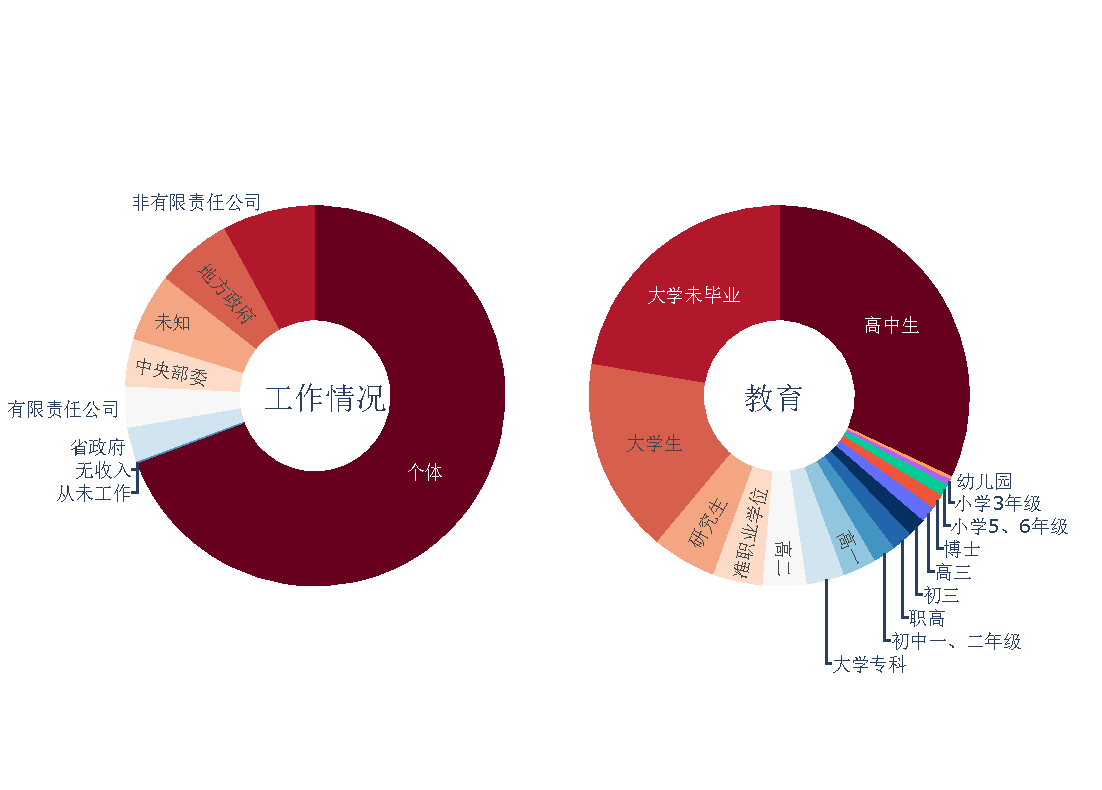
\includegraphics[width=6.0in]{images/working_education.pdf}
		\caption{}
		\label{WE}
	\end{center}
\end{figure}

\begin{figure}
	\vspace{-1cm}
	\setlength{\abovecaptionskip}{-1cm} %调整图片标题与图距离
	\setlength{\belowcaptionskip}{-0.5cm} %调整图片标题与下文距离
	\begin{center}
		\makeatletter
		\def\@captype{figure}
		\makeatother
		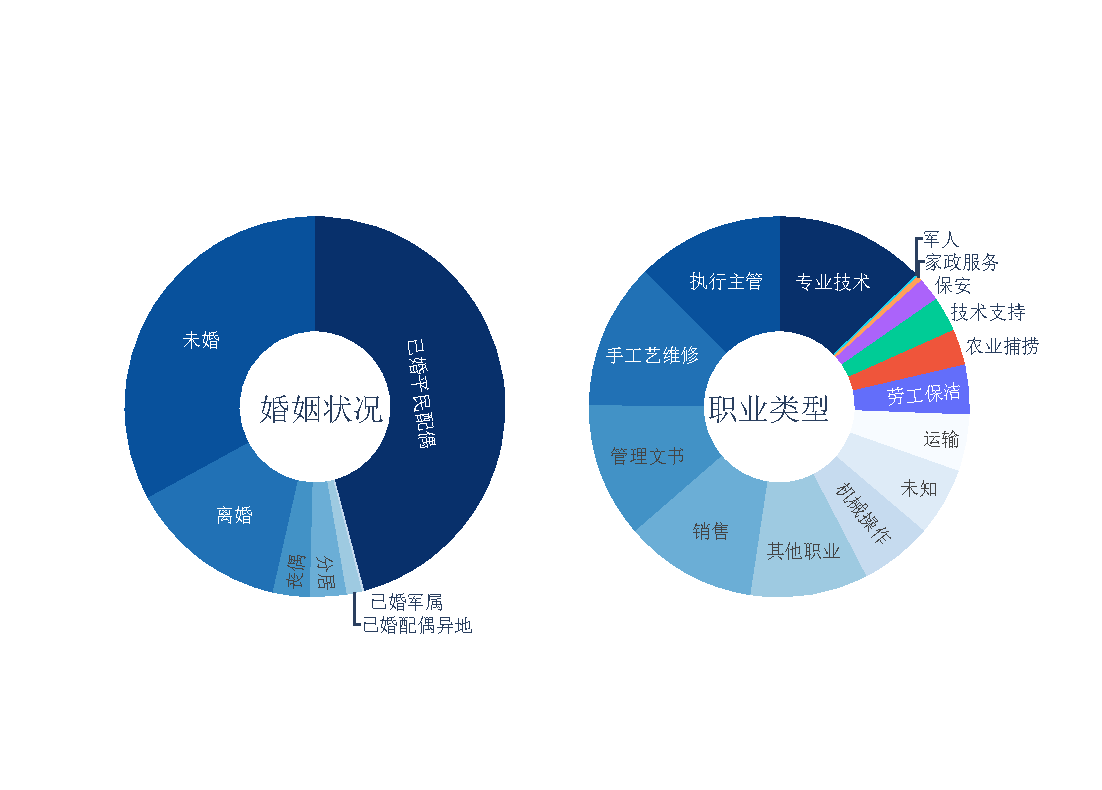
\includegraphics[width=6.0in]{images/marriage_education.pdf}
		\caption{}
		\label{ME}
	\end{center}
\end{figure}

\subsection{变量的交互作用}
本节, 我们探讨\textbf{分类变量}对与高收入$Y$概率的影响. 图 \ref{ES_to_Y}至 图\ref{} 展示了这些关系, 我们以图 \ref{} 作为分析.
\begin{figure}[htb]
	%\vspace{-3cm}
    \setlength{\abovecaptionskip}{-1cm} %调整图片标题与图距离
	\setlength{\belowcaptionskip}{-0.8cm} %调整图片标题与下文距离
	\begin{center}
		\makeatletter
		\def\@captype{figure}
		\makeatother
		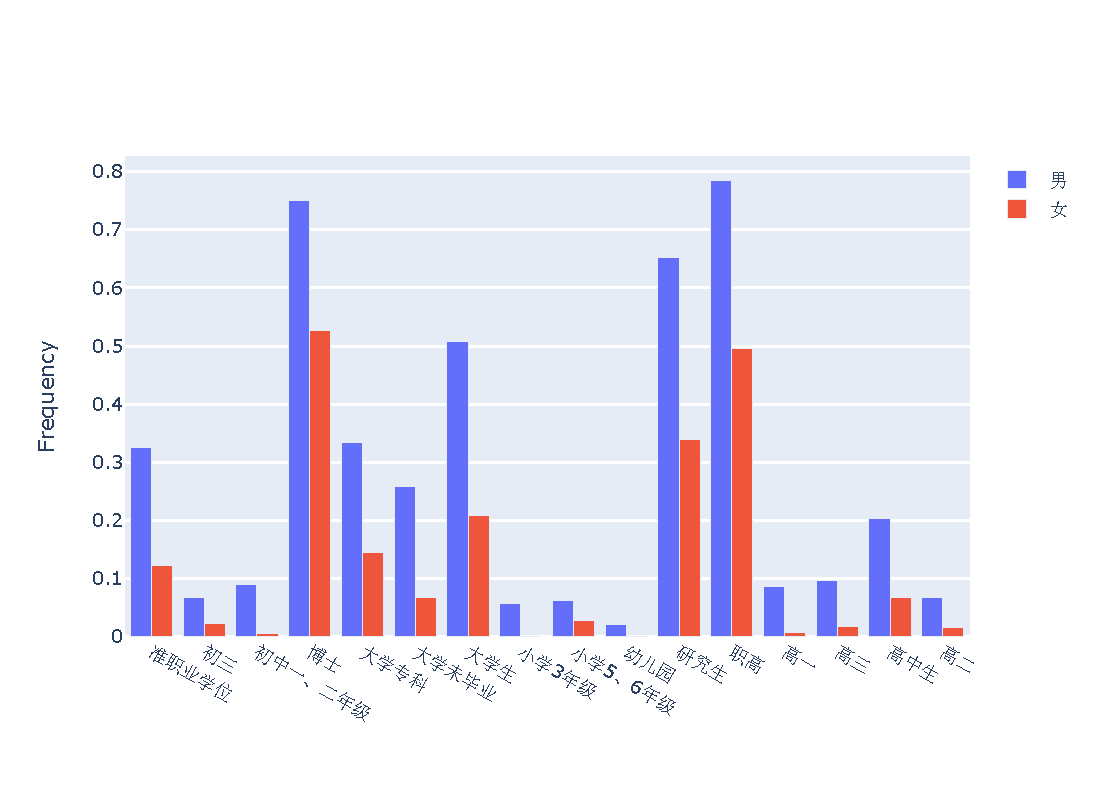
\includegraphics[width=5.0in]{images/education_sex.pdf}
		\caption{}
		\label{ES_to_Y}
	\end{center}
\end{figure}
首先值得注意的是, 在正常的体系下, 学历越高, 越容易获得高收入. 这一点从图 \ref{ES_to_Y} 中不难发现, 博士, 硕士高收入频率接近0.7.  但另一方面, 职高的收入并不比博士, 硕士低, 同时拿到准职业学位的人群也能获得不菲的收入. 这意味着如果你只是追寻获得高收入的话, 不如去读职高. \par
另一值得关注的规律是, 在所有条件下, 男性获得高收入的频率大于女性.
首先值得注意的是, 在正常的体系下, 学历越高, 越容易获得高收入. 这一点从图 \ref{ES_to_Y} 中不难发现, 博士, 硕士高收入频率接近0.7.  但另一方面, 职高的收入并不比博士, 硕士低, 同时拿到准职业学位的人群也能获得不菲的收入. 这意味着如果你只是追寻获得高收入的话, 不如去读职高. 除此之外, 可以发现, 在所有条件下, 男性获得高收入的频率大于女性. \par
事实上, 其余分类变量与性别的交互效应均满足上述规律, 但也存在例外. 从图 \ref{MS_to_Y} 中可以看到, 已婚军属女性更容易获得高收入.

\begin{figure}[htb]
	\vspace{-0cm}
	\setlength{\abovecaptionskip}{-1cm} %调整图片标题与图距离
	\setlength{\belowcaptionskip}{-1cm} %调整图片标题与下文距离
	\begin{center}
		\makeatletter
		\def\@captype{figure}
		\makeatother
		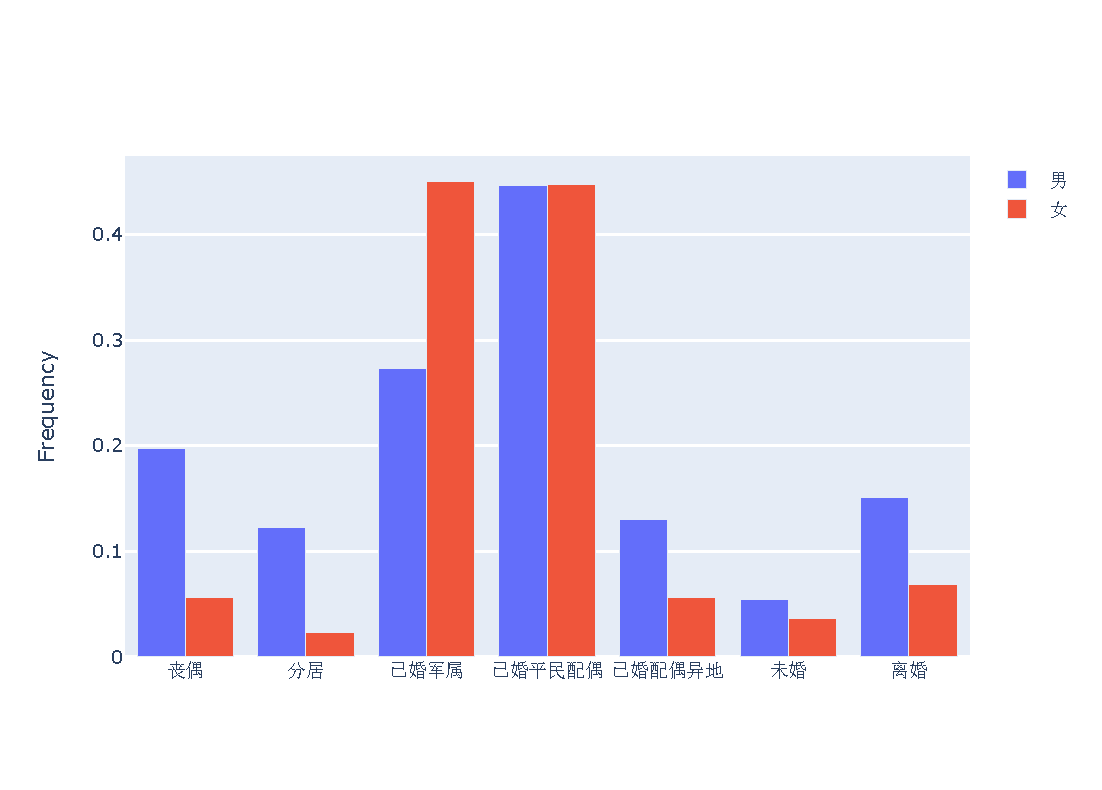
\includegraphics[width=5.0in]{images/marriage_sex.pdf}
		\caption{}
		\label{MS_to_Y}
	\end{center}
\end{figure}



\section{模型概要及数据处理}
读取数据
    \begin{tcolorbox}[breakable, size=fbox, boxrule=1pt, pad at break*=1mm,colback=cellbackground, colframe=cellborder]
	\prompt{In}{incolor}{10}{\boxspacing}
	\begin{Verbatim}[commandchars=\\\{\}]
\PY{n}{df\PYZus{}train} \PY{o}{=} \PY{n}{pd}\PY{o}{.}\PY{n}{read\PYZus{}csv}\PY{p}{(}\PY{l+s+s1}{\PYZsq{}}\PY{l+s+s1}{Train.csv}\PY{l+s+s1}{\PYZsq{}}\PY{p}{)}
\PY{n}{df\PYZus{}train}\PY{o}{.}\PY{n}{head}\PY{p}{(}\PY{p}{)}
	\end{Verbatim}
\end{tcolorbox}


\subsection{分类变量的处理}
对于分类变量的处理,尝试用One-Hot编码,将其转化为虚拟变量。
\begin{tcolorbox}[breakable, size=fbox, boxrule=1pt, pad at break*=1mm,colback=cellbackground, colframe=cellborder]
	\prompt{In}{incolor}{16}{\boxspacing}
	\begin{Verbatim}[commandchars=\\\{\}]
\PY{c+c1}{\PYZsh{} 对object类型的变量全部进行分类处理,即实现One\PYZhy{}Hot编码}
\PY{n}{int\PYZus{}ind} \PY{o}{=} \PY{n}{df\PYZus{}train}\PY{o}{.}\PY{n}{dtypes}\PY{p}{[}\PY{n}{df\PYZus{}train}\PY{o}{.}\PY{n}{dtypes}\PY{o}{!=}\PY{n+nb}{object}\PY{p}{]}\PY{o}{.}\PY{n}{index}
\PY{n}{obj\PYZus{}ind} \PY{o}{=} \PY{n}{df\PYZus{}train}\PY{o}{.}\PY{n}{dtypes}\PY{p}{[}\PY{n}{df\PYZus{}train}\PY{o}{.}\PY{n}{dtypes}\PY{o}{==}\PY{n+nb}{object}\PY{p}{]}\PY{o}{.}\PY{n}{index} \PY{c+c1}{\PYZsh{}提取types为object的列名}
\PY{k}{for} \PY{n}{val} \PY{o+ow}{in} \PY{n}{obj\PYZus{}ind}\PY{p}{:}
    \PY{n+nb}{globals}\PY{p}{(}\PY{p}{)}\PY{p}{[}\PY{l+s+s1}{\PYZsq{}}\PY{l+s+s1}{df\PYZus{}train\PYZus{}}\PY{l+s+si}{\PYZob{}\PYZcb{}}\PY{l+s+s1}{\PYZsq{}}\PY{o}{.}\PY{n}{format}\PY{p}{(}\PY{n}{val}\PY{p}{)}\PY{p}{]} \PY{o}{=} \PY{n}{pd}\PY{o}{.}\PY{n}{get\PYZus{}dummies}\PY{p}{(}\PY{n}{df\PYZus{}train}\PY{p}{[}\PY{n}{val}\PY{p}{]}\PY{p}{,}\PY{n}{prefix}\PY{o}{=}\PY{n}{val}\PY{p}{,}\PY{n}{prefix\PYZus{}sep}\PY{o}{=}\PY{l+s+s1}{\PYZsq{}}\PY{l+s+s1}{\PYZus{}}\PY{l+s+s1}{\PYZsq{}}\PY{p}{)}
	\end{Verbatim}
\end{tcolorbox}
以婚姻状况为例,我们将分类变量转化为了下述矩阵
\vspace{0.3cm}

\begin{tabular}{lrrrrrrr}
	\toprule
	{} &  丧偶 &  分居 &  已婚军属 &  已婚平民配偶 &  已婚配偶异地 &  婚未婚 &  离婚 \\
	\midrule
	0 &        0 &        0 &          0 &            1 &            0 &        0 &        0 \\
	1 &        0 &        0 &          0 &            1 &            0 &        0 &        0 \\
	2 &        0 &        0 &          0 &            0 &            0 &        1 &        0 \\
	3 &        0 &        0 &          0 &            1 &            0 &        0 &        0 \\
	4 &        0 &        0 &          0 &            0 &            0 &        1 &        0 \\
	\bottomrule
\end{tabular}
\subsection{引入非线性因素}
回归,或者预测问题,本质在于求解条件期望。以单变量情形为例,
$$
Y(\omega) = E(Y|X)(\omega) + u(\omega).
$$
其中$E(Y|X=x)$可以记作$h(x)$,由于$h(x)$的形式未知,所以我们无法给出具体的形式。通常我们假定$h(x)$具有仿射结构,此时模型也称作一元线性回归。更一般的,我们可以利用多项式去估计$h(x)$,这样做的理由是Laurent展开定理。

\begin{Theorem}[Laurent Series]{\label{LS}} 
	Suppose $f$ is analytic at an annulus of $z_0$, then f can be expressed as follows
	$$
	f(z) = \sum_{n=-\infty}^{+\infty}c_n(z-z_0)^n, \ \  z\neq z_0.
	$$
	The complex series on the right side converges uniformly on all compact sets of the annulus. Moreover, if $f$ is analytic at $z_0\in\mathbb{R}$, then 
	$$
	f(x) = \sum_{n=0}^{+\infty}c_n(x-z_0)^n.
	$$
\end{Theorem}
定理告诉我们,利用多项式函数可以对条件期望进行逼近。或者说,我们认为。
$$
E(Y|X)(\omega) \approx \beta_0 + \beta_1X(\omega) + \beta_2X(\omega)^2 + \beta_3X(\omega)^3.
$$
所以在特征工程中,我们选择加入数值型变量的二次幂以及三次幂用于刻画条件期望的非线性形式。同样的我们知道,
\begin{Theorem}[Fourier Series]{\label{FS}} 
	Suppose $f\in L^2$ , then the series given blow converges to $f$ in $L^2$. 
	$$
	\frac{a_0}{2} + \sum_{n=1}^{+\infty}a_n\cos(nx)+\sum_{n=1}^{+\infty}b_n\sin(nx) \stackrel{L^2}{\rightarrow} f(x).
	$$
	Where 
	$$
	a_n = \langle f(x),\cos(nx)\rangle, \ b_n = \langle f(x),\sin(nx)\rangle.
	$$
\end{Theorem}
可以认为
$$
E(Y|X)(\omega) \approx c_0 + c_1*cos(X(\omega))+c_2*cos(2X(\omega))+c_3*sin(X(\omega))+c_4*sin(2X(\omega))
$$
所以我们也尝试加入$cos(x)$, $cos(2x)$, $sin(x)$, $sin(2x)$ 来刻画潜在的非线性关系。\par

\subsection{变量量纲的处理}
完成对变量['年龄', '教育时间', '投资收入', '投资损失', '工作天数']分别处理后, 下面集中于对于变量量纲的处理. 我们主要考虑标准化和归一化, 并在后文对比两种处理的效果.
\begin{eqnarray*}
\vec{x}_{standard} &=& \frac{\vec{x} - E(\vec{x})}{S_{\vec{x}}} \\
\vec{x}_{min-max} &=& \frac{\vec{x} - \min \vec{x}}{ \max \vec{x} -  \min \vec{x}}
\end{eqnarray*}
标准化后的数据集记作"sndf\_train.csv", 归一化后的数据集记作"smndf\_train.csv". 
本节代码如下
    \begin{tcolorbox}[breakable, size=fbox, boxrule=1pt, pad at break*=1mm,colback=cellbackground, colframe=cellborder]
	\prompt{In}{incolor}{16}{\boxspacing}
	\begin{Verbatim}[commandchars=\\\{\}]
\PY{c+c1}{\PYZsh{} 对object类型的变量全部进行分类处理,即实现One\PYZhy{}Hot编码}
\PY{n}{int\PYZus{}ind} \PY{o}{=} \PY{n}{df\PYZus{}train}\PY{o}{.}\PY{n}{dtypes}\PY{p}{[}\PY{n}{df\PYZus{}train}\PY{o}{.}\PY{n}{dtypes}\PY{o}{!=}\PY{n+nb}{object}\PY{p}{]}\PY{o}{.}\PY{n}{index}
\PY{n}{obj\PYZus{}ind} \PY{o}{=} \PY{n}{df\PYZus{}train}\PY{o}{.}\PY{n}{dtypes}\PY{p}{[}\PY{n}{df\PYZus{}train}\PY{o}{.}\PY{n}{dtypes}\PY{o}{==}\PY{n+nb}{object}\PY{p}{]}\PY{o}{.}\PY{n}{index} \PY{c+c1}{\PYZsh{}提取types为object的列名}
\PY{k}{for} \PY{n}{val} \PY{o+ow}{in} \PY{n}{obj\PYZus{}ind}\PY{p}{:}
    \PY{n+nb}{globals}\PY{p}{(}\PY{p}{)}\PY{p}{[}\PY{l+s+s1}{\PYZsq{}}\PY{l+s+s1}{df\PYZus{}train\PYZus{}}\PY{l+s+si}{\PYZob{}\PYZcb{}}\PY{l+s+s1}{\PYZsq{}}\PY{o}{.}\PY{n}{format}\PY{p}{(}\PY{n}{val}\PY{p}{)}\PY{p}{]} \PY{o}{=} \PY{n}{pd}\PY{o}{.}\PY{n}{get\PYZus{}dummies}\PY{p}{(}\PY{n}{df\PYZus{}train}\PY{p}{[}\PY{n}{val}\PY{p}{]}\PY{p}{,}\PY{n}{prefix}\PY{o}{=}\PY{n}{val}\PY{p}{,}\PY{n}{prefix\PYZus{}sep}\PY{o}{=}\PY{l+s+s1}{\PYZsq{}}\PY{l+s+s1}{\PYZus{}}\PY{l+s+s1}{\PYZsq{}}\PY{p}{)}
	\end{Verbatim}
\end{tcolorbox}


    \begin{tcolorbox}[breakable, size=fbox, boxrule=1pt, pad at break*=1mm,colback=cellbackground, colframe=cellborder]
	\prompt{In}{incolor}{28}{\boxspacing}
	\begin{Verbatim}[commandchars=\\\{\}]
\PY{c+c1}{\PYZsh{} 引入非线性的成分}
\PY{n}{nonlinear\PYZus{}ndf\PYZus{}train} \PY{o}{=} \PY{n}{df\PYZus{}train}\PY{p}{[}\PY{n}{int\PYZus{}ind}\PY{o}{.}\PY{n}{sort\PYZus{}values}\PY{p}{(}\PY{p}{)}\PY{p}{]}
\PY{n}{temp2} \PY{o}{=} \PY{n}{nonlinear\PYZus{}ndf\PYZus{}train}\PY{o}{.}\PY{n}{iloc}\PY{p}{[}\PY{p}{:}\PY{p}{,}\PY{l+m+mi}{1}\PY{p}{:}\PY{l+m+mi}{6}\PY{p}{]}\PY{o}{.}\PY{n}{apply}\PY{p}{(}\PY{k}{lambda} \PY{n}{x}\PY{p}{:}\PY{n}{x}\PY{o}{*}\PY{o}{*}\PY{l+m+mi}{2}\PY{p}{,}\PY{n}{axis}\PY{o}{=}\PY{l+m+mi}{0}\PY{p}{)}
\PY{n}{temp3} \PY{o}{=} \PY{n}{nonlinear\PYZus{}ndf\PYZus{}train}\PY{o}{.}\PY{n}{iloc}\PY{p}{[}\PY{p}{:}\PY{p}{,}\PY{l+m+mi}{1}\PY{p}{:}\PY{l+m+mi}{6}\PY{p}{]}\PY{o}{.}\PY{n}{apply}\PY{p}{(}\PY{k}{lambda} \PY{n}{x}\PY{p}{:}\PY{n}{x}\PY{o}{*}\PY{o}{*}\PY{l+m+mi}{3}\PY{p}{,}\PY{n}{axis}\PY{o}{=}\PY{l+m+mi}{0}\PY{p}{)}
\PY{n}{temp2}\PY{o}{.}\PY{n}{columns} \PY{o}{=} \PY{n+nb}{list}\PY{p}{(}\PY{n+nb}{map}\PY{p}{(}\PY{k}{lambda} \PY{n}{x}\PY{p}{:}\PY{n}{x}\PY{o}{+}\PY{l+s+s1}{\PYZsq{}}\PY{l+s+s1}{**2}\PY{l+s+s1}{\PYZsq{}}\PY{p}{,}\PY{n+nb}{list}\PY{p}{(}\PY{n}{temp2}\PY{o}{.}\PY{n}{columns}\PY{p}{)}\PY{p}{)}\PY{p}{)}
\PY{n}{temp3}\PY{o}{.}\PY{n}{columns} \PY{o}{=} \PY{n+nb}{list}\PY{p}{(}\PY{n+nb}{map}\PY{p}{(}\PY{k}{lambda} \PY{n}{x}\PY{p}{:}\PY{n}{x}\PY{o}{+}\PY{l+s+s1}{\PYZsq{}}\PY{l+s+s1}{**3}\PY{l+s+s1}{\PYZsq{}}\PY{p}{,}\PY{n+nb}{list}\PY{p}{(}\PY{n}{temp3}\PY{o}{.}\PY{n}{columns}\PY{p}{)}\PY{p}{)}\PY{p}{)}
\PY{n}{nonlinear\PYZus{}ndf\PYZus{}train} \PY{o}{=} \PY{n}{nonlinear\PYZus{}ndf\PYZus{}train}\PY{o}{.}\PY{n}{join}\PY{p}{(}\PY{n}{temp2}\PY{p}{)}
\PY{n}{nonlinear\PYZus{}ndf\PYZus{}train} \PY{o}{=} \PY{n}{nonlinear\PYZus{}ndf\PYZus{}train}\PY{o}{.}\PY{n}{join}\PY{p}{(}\PY{n}{temp3}\PY{p}{)}
\PY{k}{for} \PY{n}{val} \PY{o+ow}{in} \PY{n}{obj\PYZus{}ind}\PY{p}{:}
\PY{n}{nonlinear\PYZus{}ndf\PYZus{}train} \PY{o}{=} \PY{n}{nonlinear\PYZus{}ndf\PYZus{}train}\PY{o}{.}\PY{n}{join}\PY{p}{(}\PY{n+nb}{globals}\PY{p}{(}\PY{p}{)}\PY{p}{[}\PY{l+s+s1}{\PYZsq{}}\PY{l+s+s1}{df\PYZus{}train\PYZus{}}\PY{l+s+si}{\PYZob{}\PYZcb{}}\PY{l+s+s1}{\PYZsq{}}\PY{o}{.}\PY{n}{format}\PY{p}{(}\PY{n}{val}\PY{p}{)}\PY{p}{]}\PY{p}{)}
\PY{n}{nonlinear\PYZus{}sndf\PYZus{}train} \PY{o}{=} \PY{n}{nonlinear\PYZus{}ndf\PYZus{}train}\PY{o}{.}\PY{n}{copy}\PY{p}{(}\PY{p}{)}
\PY{n}{nonlinear\PYZus{}smndf\PYZus{}train} \PY{o}{=} \PY{n}{nonlinear\PYZus{}ndf\PYZus{}train}\PY{o}{.}\PY{n}{copy}\PY{p}{(}\PY{p}{)}
\PY{n}{nonlinear\PYZus{}sndf\PYZus{}train}\PY{o}{.}\PY{n}{iloc}\PY{p}{[}\PY{p}{:}\PY{p}{,}\PY{l+m+mi}{1}\PY{p}{:}\PY{l+m+mi}{16}\PY{p}{]} \PY{o}{=} \PY{n}{nonlinear\PYZus{}sndf\PYZus{}train}\PY{o}{.}\PY{n}{iloc}\PY{p}{[}\PY{p}{:}\PY{p}{,}\PY{l+m+mi}{1}\PY{p}{:}\PY{l+m+mi}{16}\PY{p}{]}\PY{o}{.}\PY{n}{apply}\PY{p}{(}\PY{k}{lambda} \PY{n}{x}\PY{p}{:}\PY{p}{(}\PY{n}{x}\PY{o}{\PYZhy{}}\PY{n}{x}\PY{o}{.}\PY{n}{mean}\PY{p}{(}\PY{p}{)}\PY{p}{)}\PY{o}{/}\PY{n}{x}\PY{o}{.}\PY{n}{std}\PY{p}{(}\PY{p}{)}\PY{p}{,}\PY{n}{axis}\PY{o}{=}\PY{l+m+mi}{0}\PY{p}{)}
\PY{n}{nonlinear\PYZus{}smndf\PYZus{}train}\PY{o}{.}\PY{n}{iloc}\PY{p}{[}\PY{p}{:}\PY{p}{,}\PY{l+m+mi}{1}\PY{p}{:}\PY{l+m+mi}{16}\PY{p}{]} \PY{o}{=} \PY{n}{nonlinear\PYZus{}smndf\PYZus{}train}\PY{o}{.}\PY{n}{iloc}\PY{p}{[}\PY{p}{:}\PY{p}{,}\PY{l+m+mi}{1}\PY{p}{:}\PY{l+m+mi}{16}\PY{p}{]}\PY{o}{.}\PY{n}{apply}\PY{p}{(}\PY{k}{lambda} \PY{n}{x}\PY{p}{:}\PY{p}{(}\PY{n}{x}\PY{o}{\PYZhy{}}\PY{n}{x}\PY{o}{.}\PY{n}{min}\PY{p}{(}\PY{p}{)}\PY{p}{)}\PY{o}{/}\PY{p}{(}\PY{n}{x}\PY{o}{.}\PY{n}{max}\PY{p}{(}\PY{p}{)}\PY{o}{\PYZhy{}}\PY{n}{x}\PY{o}{.}\PY{n}{min}\PY{p}{(}\PY{p}{)}\PY{p}{)}\PY{p}{,}\PY{n}{axis}\PY{o}{=}\PY{l+m+mi}{0}\PY{p}{)}
	\end{Verbatim}
\end{tcolorbox}

\section{广义线性模型}
\subsection{模型介绍}
广义线性模型是线性模型的推广,详细介绍可见Nelder\cite{nelder1972generalized}以及Zheng \cite{zheng2000summarizing}。广义线性模型中最重要的概念是广义指数分布,我们先给出他的定义。
\begin{Definition}[Generalized Exponential Distribution]{\label{GED}} We say a random variable $Y$ follows a Generalized Exponential Distribution(GED) if the density function of 
$Y$ can be written as follows:
$$
f_Y(y) = \exp \{\ \frac{y\theta-b(\theta)}{a(\phi)}\ + c(y,\phi) \}.
$$
\end{Definition} \par
我们把服从广义指数分布的随机变量记作$Y \sim GED(\theta,\phi;a,b,c)$, 在不引起歧义的情况下,简写为$Y \sim GED(\theta,\phi)$. 事实上,初等概率论中常见的分布,如正态分布,泊松分布,二项分布,伽马分布等都属于广义指数分布族。我们将举例说明这一点。
\begin{Example}[Binomial Distribution]
二项分布属于广义指数分布族,因为
\begin{eqnarray*}
	f_Y(y) 
	&=& p^y(1-p)^{1-y} \\
	&=& e^{y\ln p} e^{(1-y) \ln 1-p}  \\
	&=& \exp\{y\ln \frac{p}{1-p}+\ln 1-p\}   
\end{eqnarray*}
在本例中,$\theta=\ln \frac{p}{1-p}$, $b(\theta)=\frac{e^{\theta}}{1+e^{\theta}}$
\end{Example}
接下来,我们将给出一般的广义线性模型参数估计的办法。事实上,广义线性模型的思想在于,我们认为随机变量$Y$可以写作, 
$$
Y = E(Y|\vec X) + Y - E(Y|\vec X)
$$
Y的条件期望与线性预测子之间可以通过链接函数$g$产生联系:
$$
g(E(Y|\vec X)) = \vec{X}^T\vec{\beta}
$$
给定一组样本,随机变量$Y$服从广义指数分布,其密度函数可以写作:
$$
f(y;\theta,\phi|\vec X=\vec x) = \exp \{\frac{y\theta-b(\theta)}{a(\phi)}\ + c(y,\phi)\}
$$
其中$\vec x$的影响体现在$\theta$中。
这样我们得到了样本对数似然函数:
$$
l(\vec \beta) = \sum_{i=1}^{n}   \frac{y_i\theta_i-b(\theta_i)}{a(\phi)}\ + c(y_i,\phi).
$$
根据复合函数求导法则,
\begin{eqnarray*}
	\frac{\partial l(\vec \beta)}{\partial \beta_j}
	 &=& \sum_{i=1}^{n} \frac{\partial l(\vec \beta)}{\partial \theta_i} \frac{d \theta_i}{d \mu_i} \frac{d \mu_i}{d \beta_j} \\ 
	 &=& \sum_{i=1}^{n} (y_i-b^{'}(\theta_i)) \frac{d \theta_i}{d \mu_i} \frac{x_{ij}}{g^{'}(\mu_j)}
\end{eqnarray*}
我们称满足$g^{'}(\mu_j) =  \frac{d \theta_i}{d \mu_i}$的$g$为典则链接函数,使用典则链接函数的好处在于能够简化参数估计的过程。对于二项分布而言,其典则链接函数为$g(\mu) = \ln \frac{\mu}{1-\mu}$, 其反函数就是我们熟知的Logistic函数,所以,Logit回归也就是当链接函数取为典则链接函数的二项回归。这也充分说明广义线性模型的广泛适用性。

\subsection{参数估计}
本节符号较多,为了便于理解,请记住如下关系式。
\begin{eqnarray*}
	E(Y|\vec X) = g^{-1}(\vec{X}^T \vec \beta)
\end{eqnarray*}
取$g$为典则链接函数,这样使得l关于$\beta$的偏导数能够得到极大化简。根据向量求导法则,我们可以得到
$$
\frac{\partial l}{\partial \vec \beta} = 
\begin{bmatrix}
	\sum_{i=1}^{n} \frac{y_i-E(Y|\vec{x}_i)}{a(\phi)}x_{i1}\\ 
	\sum_{i=1}^{n} \frac{y_i-E(Y|\vec{x}_i)}{a(\phi)}x_{i2} \\ 
	\vdots \\ 
	\sum_{i=1}^{n} \frac{y_i-E(Y|\vec{x}_i)}{a(\phi)}x_{ip+1}
\end{bmatrix}
= \vec 0 
$$
事实上,这与线性模型中的"正规方程组"形式上是相同的,通过求解上述非线性方程组,即可得到$\beta$的估计值。接下来我们借助fisher信息矩阵给出参数估计量的协方差矩阵。
\begin{Definition}[Fisher Information Matrix]{\label{fim}} The Fisher information matrix of multiple parameters is defined by 
$$
I_1(\vec{\beta}) = E(\frac{\partial \ln f(X,\vec \beta)}{\partial \vec \beta})(\frac{\partial \ln f(X,\vec \beta)}{\partial \vec \beta})^T
$$
Easy to verify that the fisher information matrix is equal to minus the expectation of Hessian matrix of $\ln f(X,\vec{\beta})$.
通过计算可以得到,当连接函数为典则链接函数时,
$$
I_1(\vec{\beta}) = 
\begin{bmatrix}
	1 & X_{11} & \cdots & X_{1p} \\
	1 & X_{21} & \cdots & X_{2p} \\
	\vdots & \vdots & &\vdots \\
	1 & X_{n1} & \cdots & X_{np} \\
\end{bmatrix}^T
\begin{bmatrix}
	\frac{1}{g^{'}(\mu_1)} & 0 & \cdots &0 \\
	0 &\frac{1}{g^{'}(\mu_2)} & \cdots & 0 \\
	\vdots & \vdots & &\vdots \\
	0 & 0 & \cdots & \frac{1}{g^{'}(\mu_2)} \\
\end{bmatrix}
\begin{bmatrix}
	1 & X_{11} & \cdots & X_{1p} \\
	1 & X_{21} & \cdots & X_{2p} \\
	\vdots & \vdots & &\vdots \\
	1 & X_{n1} & \cdots & X_{np} \\
\end{bmatrix}
$$
我们不加证明的给出
\begin{Theorem}{The asymptomatic property of MLE}
	$$
\sqrt n(\vec{\hat \beta}_{MLE}-\vec{\beta}) \simeq \mathcal{N}(0,I_1^{-1}(\vec{\beta}))
$$
\end{Theorem}

\end{Definition} 
\section{预测}
\subsection{分类器}
为了更方便的使用各种模型,本文选择先定义一个叫做Classifiers的类,具体如下。该class中定义了数十种分类器,并计算了auc等指标,为后续参数调整,更换模型,数据集等提供了极大便利。
    \begin{tcolorbox}[breakable, size=fbox, boxrule=1pt, pad at break*=1mm,colback=cellbackground, colframe=cellborder]
	\prompt{In}{incolor}{ }{\boxspacing}
	\begin{Verbatim}[commandchars=\\\{\}]
\PY{k}{class} \PY{n+nc}{Classifiers}\PY{p}{(}\PY{p}{)}\PY{p}{:}
\PY{n}{details} \PY{o}{=} \PY{p}{[}\PY{l+s+s1}{\PYZsq{}}\PY{l+s+s1}{LogisticRegression}\PY{l+s+s1}{\PYZsq{}}\PY{p}{,}\PY{l+s+s1}{\PYZsq{}}\PY{l+s+s1}{XGBClassifier}\PY{l+s+s1}{\PYZsq{}}\PY{p}{,}\PY{l+s+s1}{\PYZsq{}}\PY{l+s+s1}{GradientBoostingClassifier}\PY{l+s+s1}{\PYZsq{}}\PY{p}{,}\PY{l+s+s1}{\PYZsq{}}\PY{l+s+s1}{AdaBoostClassifier}\PY{l+s+s1}{\PYZsq{}}\PY{p}{,}
\PY{l+s+s1}{\PYZsq{}}\PY{l+s+s1}{RandomForestClassifier}\PY{l+s+s1}{\PYZsq{}}\PY{p}{,}\PY{l+s+s1}{\PYZsq{}}\PY{l+s+s1}{KNeighborsClassifier}\PY{l+s+s1}{\PYZsq{}}\PY{p}{,}\PY{l+s+s1}{\PYZsq{}}\PY{l+s+s1}{DecisionTreeClassifier}\PY{l+s+s1}{\PYZsq{}}\PY{p}{,}\PY{l+s+s1}{\PYZsq{}}\PY{l+s+s1}{MLPsClassifier}\PY{l+s+s1}{\PYZsq{}}\PY{p}{,}\PY{l+s+s1}{\PYZsq{}}\PY{l+s+s1}{CatBoostClassifier}\PY{l+s+s1}{\PYZsq{}}\PY{p}{]}

\PY{k}{def} \PY{n+nf+fm}{\PYZus{}\PYZus{}init\PYZus{}\PYZus{}}\PY{p}{(}\PY{n+nb+bp}{self}\PY{p}{,}\PY{n}{class\PYZus{}model}\PY{p}{)}\PY{p}{:}
\PY{n+nb+bp}{self}\PY{o}{.}\PY{n}{model\PYZus{}class} \PY{o}{=} \PY{n}{class\PYZus{}model}\PY{p}{(}\PY{p}{)}
\PY{n+nb+bp}{self}\PY{o}{.}\PY{n}{model\PYZus{}name} \PY{o}{=} \PY{n+nb}{str}\PY{p}{(}\PY{n+nb+bp}{self}\PY{o}{.}\PY{n}{model\PYZus{}class}\PY{p}{)}\PY{o}{.}\PY{n}{split}\PY{p}{(}\PY{l+s+s1}{\PYZsq{}}\PY{l+s+s1}{(}\PY{l+s+s1}{\PYZsq{}}\PY{p}{)}\PY{p}{[}\PY{l+m+mi}{0}\PY{p}{]}
\PY{c+c1}{\PYZsh{}self.model\PYZus{}params = Classifiers\PYZus{}dict[self.model\PYZus{}name]}
\PY{c+c1}{\PYZsh{} 构建常用参数字典}
\PY{k}{def} \PY{n+nf}{param\PYZus{}dict}\PY{p}{(}\PY{n+nb+bp}{self}\PY{p}{)}\PY{p}{:}
\PY{n+nb}{print}\PY{p}{(}\PY{l+s+s1}{\PYZsq{}}\PY{l+s+s1}{1}\PY{l+s+s1}{\PYZsq{}}\PY{p}{)}
\PY{k}{def} \PY{n+nf}{setmodelparam}\PY{p}{(}\PY{n+nb+bp}{self}\PY{p}{,}\PY{n}{class\PYZus{}model}\PY{p}{,}\PY{o}{*}\PY{n}{args}\PY{p}{,}\PY{o}{*}\PY{o}{*}\PY{n}{kwargs}\PY{p}{)}\PY{p}{:}
\PY{n+nb+bp}{self}\PY{o}{.}\PY{n}{model\PYZus{}paramed} \PY{o}{=} \PY{n}{class\PYZus{}model}\PY{p}{(}\PY{o}{*}\PY{n}{args}\PY{p}{,}\PY{o}{*}\PY{o}{*}\PY{n}{kwargs}\PY{p}{)}

\PY{k}{def} \PY{n+nf}{setdata}\PY{p}{(}\PY{n+nb+bp}{self}\PY{p}{,}\PY{n}{X}\PY{p}{,}\PY{n}{Y}\PY{p}{,}\PY{n}{test\PYZus{}size}\PY{o}{=}\PY{l+m+mf}{0.3}\PY{p}{,}\PY{n}{random\PYZus{}state}\PY{o}{=}\PY{l+m+mi}{0}\PY{p}{)}\PY{p}{:}
\PY{n+nb+bp}{self}\PY{o}{.}\PY{n}{Xdata} \PY{o}{=} \PY{n}{X}
\PY{n+nb+bp}{self}\PY{o}{.}\PY{n}{Ydata} \PY{o}{=} \PY{n}{Y}
\PY{n+nb+bp}{self}\PY{o}{.}\PY{n}{X\PYZus{}train}\PY{p}{,} \PY{n+nb+bp}{self}\PY{o}{.}\PY{n}{X\PYZus{}test}\PY{p}{,} \PY{n+nb+bp}{self}\PY{o}{.}\PY{n}{Y\PYZus{}train}\PY{p}{,} \PY{n+nb+bp}{self}\PY{o}{.}\PY{n}{Y\PYZus{}test} \PY{o}{=}  \PY{n}{train\PYZus{}test\PYZus{}split}\PY{p}{(}\PY{n}{X}\PY{p}{,}\PY{n}{Y}\PY{p}{,} \PY{n}{test\PYZus{}size}\PY{o}{=}\PY{n}{test\PYZus{}size}\PY{p}{,}\PY{n}{random\PYZus{}state}\PY{o}{=}\PY{n}{rn}\PY{p}{)}
\PY{n+nb+bp}{self}\PY{o}{.}\PY{n}{X\PYZus{}train\PYZus{}abs}\PY{p}{,} \PY{n+nb+bp}{self}\PY{o}{.}\PY{n}{X\PYZus{}valid}\PY{p}{,} \PY{n+nb+bp}{self}\PY{o}{.}\PY{n}{Y\PYZus{}train\PYZus{}abs}\PY{p}{,} \PY{n+nb+bp}{self}\PY{o}{.}\PY{n}{Y\PYZus{}valid} \PY{o}{=}  \PY{n}{train\PYZus{}test\PYZus{}split}\PY{p}{(}\PY{n+nb+bp}{self}\PY{o}{.}\PY{n}{X\PYZus{}train}\PY{p}{,}\PY{n+nb+bp}{self}\PY{o}{.}\PY{n}{Y\PYZus{}train}\PY{p}{,} \PY{n}{test\PYZus{}size}\PY{o}{=}\PY{l+m+mf}{0.2}\PY{p}{,}\PY{n}{random\PYZus{}state}\PY{o}{=}\PY{n}{rn}\PY{p}{)}

\PY{k}{def} \PY{n+nf}{fit\PYZus{}model}\PY{p}{(}\PY{n+nb+bp}{self}\PY{p}{,}\PY{n}{X\PYZus{}train}\PY{o}{=}\PY{p}{[}\PY{k+kc}{None}\PY{p}{]}\PY{p}{,}\PY{n}{Y\PYZus{}train}\PY{o}{=}\PY{p}{[}\PY{k+kc}{None}\PY{p}{]}\PY{p}{,}\PY{n}{cv}\PY{o}{=}\PY{l+m+mi}{0}\PY{p}{,}\PY{o}{*}\PY{n}{kargs}\PY{p}{,}\PY{o}{*}\PY{o}{*}\PY{n}{kwargs}\PY{p}{)}\PY{p}{:}
\PY{k}{if} \PY{n+nb}{list}\PY{p}{(}\PY{n}{Y\PYZus{}train}\PY{p}{)}\PY{p}{[}\PY{l+m+mi}{0}\PY{p}{]} \PY{o}{==} \PY{k+kc}{None}\PY{p}{:}
\PY{n}{X\PYZus{}train}\PY{p}{,} \PY{n}{Y\PYZus{}train} \PY{o}{=} \PY{n+nb+bp}{self}\PY{o}{.}\PY{n}{X\PYZus{}train}\PY{p}{,}\PY{n+nb+bp}{self}\PY{o}{.}\PY{n}{Y\PYZus{}train}
\PY{n+nb+bp}{self}\PY{o}{.}\PY{n}{model\PYZus{}fitted} \PY{o}{=} \PY{n+nb+bp}{self}\PY{o}{.}\PY{n}{model\PYZus{}paramed}\PY{o}{.}\PY{n}{fit}\PY{p}{(}\PY{n}{X\PYZus{}train}\PY{p}{,}\PY{n}{Y\PYZus{}train}\PY{p}{,}\PY{o}{*}\PY{n}{kargs}\PY{p}{,}\PY{o}{*}\PY{o}{*}\PY{n}{kwargs}\PY{p}{)}
\PY{k}{if} \PY{n}{cv} \PY{o}{\PYZgt{}} \PY{l+m+mi}{0}\PY{p}{:}
\PY{n+nb+bp}{self}\PY{o}{.}\PY{n}{Y\PYZus{}train\PYZus{}predict\PYZus{}CV} \PY{o}{=} \PY{n}{cross\PYZus{}val\PYZus{}predict}\PY{p}{(}\PY{n+nb+bp}{self}\PY{o}{.}\PY{n}{model\PYZus{}fitted}\PY{p}{,}\PY{n+nb+bp}{self}\PY{o}{.}\PY{n}{X\PYZus{}train}\PY{p}{,}\PY{n+nb+bp}{self}\PY{o}{.}\PY{n}{Y\PYZus{}train}\PY{p}{,}\PY{n}{cv}\PY{o}{=}\PY{n}{cv}\PY{p}{)}
\PY{n+nb+bp}{self}\PY{o}{.}\PY{n}{Y\PYZus{}test\PYZus{}predict\PYZus{}CV} \PY{o}{=} \PY{n}{cross\PYZus{}val\PYZus{}predict}\PY{p}{(}\PY{n+nb+bp}{self}\PY{o}{.}\PY{n}{model\PYZus{}fitted}\PY{p}{,}\PY{n+nb+bp}{self}\PY{o}{.}\PY{n}{X\PYZus{}test}\PY{p}{,}\PY{n+nb+bp}{self}\PY{o}{.}\PY{n}{Y\PYZus{}test}\PY{p}{,}\PY{n}{cv}\PY{o}{=}\PY{n}{cv}\PY{p}{)}
\PY{n+nb+bp}{self}\PY{o}{.}\PY{n}{Y\PYZus{}test\PYZus{}prob\PYZus{}CV} \PY{o}{=} \PY{n}{cross\PYZus{}val\PYZus{}predict}\PY{p}{(}\PY{n+nb+bp}{self}\PY{o}{.}\PY{n}{model\PYZus{}fitted}\PY{p}{,}\PY{n+nb+bp}{self}\PY{o}{.}\PY{n}{X\PYZus{}test}\PY{p}{,}\PY{n+nb+bp}{self}\PY{o}{.}\PY{n}{Y\PYZus{}test}\PY{p}{,}\PY{n}{cv}\PY{o}{=}\PY{n}{cv}\PY{p}{,}\PY{n}{method}\PY{o}{=}\PY{l+s+s1}{\PYZsq{}}\PY{l+s+s1}{predict\PYZus{}proba}\PY{l+s+s1}{\PYZsq{}}\PY{p}{)}
\PY{n+nb+bp}{self}\PY{o}{.}\PY{n}{fpr\PYZus{}CV}\PY{p}{,}\PY{n+nb+bp}{self}\PY{o}{.}\PY{n}{tpr\PYZus{}CV}\PY{p}{,}\PY{n+nb+bp}{self}\PY{o}{.}\PY{n}{thresholds\PYZus{}CV} \PY{o}{=} \PY{n}{roc\PYZus{}curve}\PY{p}{(}\PY{n+nb+bp}{self}\PY{o}{.}\PY{n}{Y\PYZus{}test}\PY{p}{,}\PY{n+nb+bp}{self}\PY{o}{.}\PY{n}{Y\PYZus{}test\PYZus{}prob\PYZus{}CV}\PY{p}{[}\PY{p}{:}\PY{p}{,}\PY{l+m+mi}{1}\PY{p}{]}\PY{p}{)}
\PY{n+nb+bp}{self}\PY{o}{.}\PY{n}{auc\PYZus{}CV} \PY{o}{=} \PY{n}{auc}\PY{p}{(}\PY{n+nb+bp}{self}\PY{o}{.}\PY{n}{fpr\PYZus{}CV}\PY{p}{,}\PY{n+nb+bp}{self}\PY{o}{.}\PY{n}{tpr\PYZus{}CV}\PY{p}{)} 
\PY{k}{else}\PY{p}{:}
\PY{n+nb+bp}{self}\PY{o}{.}\PY{n}{Y\PYZus{}train\PYZus{}predict} \PY{o}{=} \PY{n+nb+bp}{self}\PY{o}{.}\PY{n}{model\PYZus{}fitted}\PY{o}{.}\PY{n}{predict}\PY{p}{(}\PY{n+nb+bp}{self}\PY{o}{.}\PY{n}{X\PYZus{}train}\PY{p}{)}
\PY{n+nb+bp}{self}\PY{o}{.}\PY{n}{Y\PYZus{}test\PYZus{}predict} \PY{o}{=} \PY{n+nb+bp}{self}\PY{o}{.}\PY{n}{model\PYZus{}fitted}\PY{o}{.}\PY{n}{predict}\PY{p}{(}\PY{n+nb+bp}{self}\PY{o}{.}\PY{n}{X\PYZus{}test}\PY{p}{)}
\PY{n+nb+bp}{self}\PY{o}{.}\PY{n}{Y\PYZus{}test\PYZus{}prob} \PY{o}{=} \PY{n+nb+bp}{self}\PY{o}{.}\PY{n}{model\PYZus{}fitted}\PY{o}{.}\PY{n}{predict\PYZus{}proba}\PY{p}{(}\PY{n+nb+bp}{self}\PY{o}{.}\PY{n}{X\PYZus{}test}\PY{p}{)}
\PY{n+nb+bp}{self}\PY{o}{.}\PY{n}{fpr}\PY{p}{,}\PY{n+nb+bp}{self}\PY{o}{.}\PY{n}{tpr}\PY{p}{,}\PY{n+nb+bp}{self}\PY{o}{.}\PY{n}{thresholds} \PY{o}{=} \PY{n}{roc\PYZus{}curve}\PY{p}{(}\PY{n+nb+bp}{self}\PY{o}{.}\PY{n}{Y\PYZus{}test}\PY{p}{,}\PY{n+nb+bp}{self}\PY{o}{.}\PY{n}{Y\PYZus{}test\PYZus{}prob}\PY{p}{[}\PY{p}{:}\PY{p}{,}\PY{l+m+mi}{1}\PY{p}{]}\PY{p}{)}
\PY{n+nb+bp}{self}\PY{o}{.}\PY{n}{auc} \PY{o}{=} \PY{n}{auc}\PY{p}{(}\PY{n+nb+bp}{self}\PY{o}{.}\PY{n}{fpr}\PY{p}{,}\PY{n+nb+bp}{self}\PY{o}{.}\PY{n}{tpr}\PY{p}{)}

\PY{k}{def} \PY{n+nf}{roc\PYZus{}curve\PYZus{}plot}\PY{p}{(}\PY{n+nb+bp}{self}\PY{p}{,}\PY{n}{filepath}\PY{p}{,}\PY{n}{dpi}\PY{o}{=}\PY{l+m+mi}{400}\PY{p}{,}\PY{n}{figsave}\PY{o}{=}\PY{k+kc}{False}\PY{p}{)}\PY{p}{:}
\PY{n}{plt}\PY{o}{.}\PY{n}{style}\PY{o}{.}\PY{n}{use}\PY{p}{(}\PY{p}{[}\PY{l+s+s1}{\PYZsq{}}\PY{l+s+s1}{nature}\PY{l+s+s1}{\PYZsq{}}\PY{p}{,}\PY{l+s+s1}{\PYZsq{}}\PY{l+s+s1}{science}\PY{l+s+s1}{\PYZsq{}}\PY{p}{]}\PY{p}{)}
\PY{n}{plt}\PY{o}{.}\PY{n}{figure}\PY{p}{(}\PY{n}{figsize}\PY{o}{=}\PY{p}{(}\PY{l+m+mi}{8}\PY{p}{,}\PY{l+m+mi}{7}\PY{p}{)}\PY{p}{)}
\PY{n}{plt}\PY{o}{.}\PY{n}{plot}\PY{p}{(}\PY{n+nb+bp}{self}\PY{o}{.}\PY{n}{fpr}\PY{p}{,} \PY{n+nb+bp}{self}\PY{o}{.}\PY{n}{tpr}\PY{p}{,} \PY{n}{lw}\PY{o}{=}\PY{l+m+mi}{2}\PY{p}{,} \PY{n}{alpha}\PY{o}{=}\PY{l+m+mf}{.6}\PY{p}{)}
\PY{n}{plt}\PY{o}{.}\PY{n}{plot}\PY{p}{(}\PY{p}{[}\PY{l+m+mi}{0}\PY{p}{,} \PY{l+m+mi}{1}\PY{p}{]}\PY{p}{,} \PY{p}{[}\PY{l+m+mi}{0}\PY{p}{,} \PY{l+m+mi}{1}\PY{p}{]}\PY{p}{,} \PY{n}{lw}\PY{o}{=}\PY{l+m+mi}{2}\PY{p}{,} \PY{n}{linestyle}\PY{o}{=}\PY{l+s+s2}{\PYZdq{}}\PY{l+s+s2}{\PYZhy{}\PYZhy{}}\PY{l+s+s2}{\PYZdq{}}\PY{p}{)}
\PY{n}{plt}\PY{o}{.}\PY{n}{xlim}\PY{p}{(}\PY{p}{[}\PY{o}{\PYZhy{}}\PY{l+m+mf}{0.05}\PY{p}{,} \PY{l+m+mi}{1}\PY{p}{]}\PY{p}{)}
\PY{n}{plt}\PY{o}{.}\PY{n}{ylim}\PY{p}{(}\PY{p}{[}\PY{o}{\PYZhy{}}\PY{l+m+mf}{0.005}\PY{p}{,} \PY{l+m+mf}{1.05}\PY{p}{]}\PY{p}{)}
\PY{n}{plt}\PY{o}{.}\PY{n}{xlabel}\PY{p}{(}\PY{l+s+s2}{\PYZdq{}}\PY{l+s+s2}{False Positive Rate}\PY{l+s+s2}{\PYZdq{}}\PY{p}{,}\PY{n}{fontsize}\PY{o}{=}\PY{l+m+mi}{10}\PY{p}{)}
\PY{n}{plt}\PY{o}{.}\PY{n}{ylabel}\PY{p}{(}\PY{l+s+s2}{\PYZdq{}}\PY{l+s+s2}{True Positive Rate}\PY{l+s+s2}{\PYZdq{}}\PY{p}{,}\PY{n}{fontsize}\PY{o}{=}\PY{l+m+mi}{10}\PY{p}{)}
\PY{n}{plt}\PY{o}{.}\PY{n}{title}\PY{p}{(}\PY{l+s+s2}{\PYZdq{}}\PY{l+s+s2}{ROC curve}\PY{l+s+s2}{\PYZdq{}}\PY{p}{,}\PY{n}{fontsize}\PY{o}{=}\PY{l+m+mi}{12}\PY{p}{)}
\PY{n}{plt}\PY{o}{.}\PY{n}{legend}\PY{p}{(}\PY{p}{[}\PY{l+s+s2}{\PYZdq{}}\PY{l+s+s2}{(AUC }\PY{l+s+si}{\PYZob{}:.4f\PYZcb{}}\PY{l+s+s2}{)}\PY{l+s+s2}{\PYZdq{}}\PY{o}{.}\PY{n}{format}\PY{p}{(}\PY{n+nb+bp}{self}\PY{o}{.}\PY{n}{auc}\PY{p}{)}\PY{p}{]}\PY{p}{,} \PY{n}{fontsize}\PY{o}{=}\PY{l+m+mi}{8}\PY{p}{,} \PY{n}{loc}\PY{o}{=}\PY{l+m+mi}{2}\PY{p}{)}
\PY{k}{if} \PY{n}{figsave}\PY{o}{==}\PY{k+kc}{True}\PY{p}{:}
\PY{n}{plt}\PY{o}{.}\PY{n}{savefig}\PY{p}{(}\PY{n}{filepath}\PY{p}{,} \PY{n}{dpi}\PY{o}{=}\PY{n}{dpi}\PY{p}{,} \PY{n}{bbox\PYZus{}inches}\PY{o}{=}\PY{l+s+s1}{\PYZsq{}}\PY{l+s+s1}{tight}\PY{l+s+s1}{\PYZsq{}}\PY{p}{,}\PY{n+nb}{format}\PY{o}{=}\PY{l+s+s2}{\PYZdq{}}\PY{l+s+s2}{pdf}\PY{l+s+s2}{\PYZdq{}}\PY{p}{)} 
\PY{n}{plt}\PY{o}{.}\PY{n}{show}\PY{p}{(}\PY{p}{)}\PY{p}{;}

\PY{k}{def} \PY{n+nf}{confusion\PYZus{}matrix\PYZus{}train}\PY{p}{(}\PY{n+nb+bp}{self}\PY{p}{,}\PY{n}{cv}\PY{o}{=}\PY{l+m+mi}{0}\PY{p}{)}\PY{p}{:}
\PY{k}{if} \PY{n}{cv} \PY{o}{\PYZgt{}} \PY{l+m+mi}{0}\PY{p}{:}
\PY{c+c1}{\PYZsh{}print(\PYZdq{}Confusion matrix (training):\PYZbs{}n \PYZob{}0\PYZcb{}\PYZbs{}n\PYZdq{}.format(confusion\PYZus{}matrix(self.Y\PYZus{}train, self.Y\PYZus{}train\PYZus{}predict\PYZus{}CV)))}
\PY{n+nb}{print}\PY{p}{(}\PY{l+s+s2}{\PYZdq{}}\PY{l+s+s2}{Classification report (training):}\PY{l+s+se}{\PYZbs{}n}\PY{l+s+s2}{ }\PY{l+s+si}{\PYZob{}0\PYZcb{}}\PY{l+s+s2}{\PYZdq{}}\PY{o}{.}\PY{n}{format}\PY{p}{(}\PY{n}{classification\PYZus{}report}\PY{p}{(}\PY{n+nb+bp}{self}\PY{o}{.}\PY{n}{Y\PYZus{}train}\PY{p}{,} \PY{n+nb+bp}{self}\PY{o}{.}\PY{n}{Y\PYZus{}train\PYZus{}predict\PYZus{}CV}\PY{p}{)}\PY{p}{)}\PY{p}{)}           
\PY{k}{else}\PY{p}{:}
\PY{c+c1}{\PYZsh{}print(\PYZdq{}Confusion matrix (training):\PYZbs{}n \PYZob{}0\PYZcb{}\PYZbs{}n\PYZdq{}.format(confusion\PYZus{}matrix(self.Y\PYZus{}train, self.Y\PYZus{}train\PYZus{}predict)))}
\PY{n+nb}{print}\PY{p}{(}\PY{l+s+s2}{\PYZdq{}}\PY{l+s+s2}{Classification report (training):}\PY{l+s+se}{\PYZbs{}n}\PY{l+s+s2}{ }\PY{l+s+si}{\PYZob{}0\PYZcb{}}\PY{l+s+s2}{\PYZdq{}}\PY{o}{.}\PY{n}{format}\PY{p}{(}\PY{n}{classification\PYZus{}report}\PY{p}{(}\PY{n+nb+bp}{self}\PY{o}{.}\PY{n}{Y\PYZus{}train}\PY{p}{,} \PY{n+nb+bp}{self}\PY{o}{.}\PY{n}{Y\PYZus{}train\PYZus{}predict}\PY{p}{)}\PY{p}{)}\PY{p}{)}                       

\PY{k}{def} \PY{n+nf}{confusion\PYZus{}matrix\PYZus{}test}\PY{p}{(}\PY{n+nb+bp}{self}\PY{p}{,}\PY{n}{cv}\PY{o}{=}\PY{l+m+mi}{0}\PY{p}{)}\PY{p}{:}
\PY{k}{if} \PY{n}{cv} \PY{o}{\PYZgt{}} \PY{l+m+mi}{0}\PY{p}{:}
\PY{c+c1}{\PYZsh{}print(\PYZdq{}Confusion matrix (testing):\PYZbs{}n \PYZob{}0\PYZcb{}\PYZbs{}n\PYZdq{}.format(confusion\PYZus{}matrix(self.Y\PYZus{}test, self.Y\PYZus{}test\PYZus{}predict\PYZus{}CV)))}
\PY{n+nb}{print}\PY{p}{(}\PY{l+s+s2}{\PYZdq{}}\PY{l+s+s2}{Classification report (testing):}\PY{l+s+se}{\PYZbs{}n}\PY{l+s+s2}{ }\PY{l+s+si}{\PYZob{}0\PYZcb{}}\PY{l+s+s2}{\PYZdq{}}\PY{o}{.}\PY{n}{format}\PY{p}{(}\PY{n}{classification\PYZus{}report}\PY{p}{(}\PY{n+nb+bp}{self}\PY{o}{.}\PY{n}{Y\PYZus{}test}\PY{p}{,} \PY{n+nb+bp}{self}\PY{o}{.}\PY{n}{Y\PYZus{}test\PYZus{}predict\PYZus{}CV}\PY{p}{)}\PY{p}{)}\PY{p}{)}           
\PY{k}{else}\PY{p}{:}
\PY{c+c1}{\PYZsh{}print(\PYZdq{}Confusion matrix (testing):\PYZbs{}n \PYZob{}0\PYZcb{}\PYZbs{}n\PYZdq{}.format(confusion\PYZus{}matrix(self.Y\PYZus{}test, self.Y\PYZus{}test\PYZus{}predict)))}
\PY{n+nb}{print}\PY{p}{(}\PY{l+s+s2}{\PYZdq{}}\PY{l+s+s2}{Classification report (testing):}\PY{l+s+se}{\PYZbs{}n}\PY{l+s+s2}{ }\PY{l+s+si}{\PYZob{}0\PYZcb{}}\PY{l+s+s2}{\PYZdq{}}\PY{o}{.}\PY{n}{format}\PY{p}{(}\PY{n}{classification\PYZus{}report}\PY{p}{(}\PY{n+nb+bp}{self}\PY{o}{.}\PY{n}{Y\PYZus{}test}\PY{p}{,} \PY{n+nb+bp}{self}\PY{o}{.}\PY{n}{Y\PYZus{}test\PYZus{}predict}\PY{p}{)}\PY{p}{)}\PY{p}{)}     

\PY{k}{def} \PY{n+nf}{details\PYZus{}print}\PY{p}{(}\PY{n+nb+bp}{self}\PY{p}{)}\PY{p}{:}
\PY{k}{for} \PY{n}{i} \PY{o+ow}{in} \PY{n+nb+bp}{self}\PY{o}{.}\PY{n}{details}\PY{p}{:}
\PY{n+nb}{print}\PY{p}{(}\PY{n}{i}\PY{o}{+}\PY{l+s+s1}{\PYZsq{}}\PY{l+s+se}{\PYZbs{}n}\PY{l+s+s1}{\PYZsq{}}\PY{o}{+}\PY{l+s+s1}{\PYZsq{}}\PY{l+s+s1}{\PYZhy{}\PYZhy{}\PYZhy{}\PYZhy{}\PYZhy{}\PYZhy{}\PYZhy{}\PYZhy{}\PYZhy{}\PYZhy{}\PYZhy{}\PYZhy{}\PYZhy{}\PYZhy{}\PYZhy{}\PYZhy{}\PYZhy{}\PYZhy{}\PYZhy{}\PYZhy{}\PYZhy{}\PYZhy{}\PYZhy{}\PYZhy{}\PYZhy{}\PYZhy{}\PYZhy{}\PYZhy{}\PYZhy{}\PYZhy{}\PYZhy{}\PYZhy{}\PYZhy{}}\PY{l+s+s1}{\PYZsq{}}\PY{p}{)}
\PY{k}{def} \PY{n+nf}{learning\PYZus{}curve\PYZus{}plot}\PY{p}{(}\PY{n+nb+bp}{self}\PY{p}{,}\PY{n}{nmax}\PY{o}{=}\PY{l+m+mi}{20}\PY{p}{)}\PY{p}{:}
\PY{n+nb+bp}{self}\PY{o}{.}\PY{n}{diagnose\PYZus{}train\PYZus{}size}\PY{p}{,}\PY{n+nb+bp}{self}\PY{o}{.}\PY{n}{diagnose\PYZus{}train\PYZus{}loss}\PY{p}{,}\PY{n+nb+bp}{self}\PY{o}{.}\PY{n}{diagnose\PYZus{}test\PYZus{}loss} \PY{o}{=} \PY{n}{learning\PYZus{}curve}\PY{p}{(}\PY{n+nb+bp}{self}\PY{o}{.}\PY{n}{model\PYZus{}fitted}\PY{p}{,}\PY{n+nb+bp}{self}\PY{o}{.}\PY{n}{Xdata}\PY{p}{,}\PY{n+nb+bp}{self}\PY{o}{.}\PY{n}{Ydata}\PY{p}{,}
\PY{n}{scoring}\PY{o}{=}\PY{l+s+s1}{\PYZsq{}}\PY{l+s+s1}{neg\PYZus{}mean\PYZus{}squared\PYZus{}error}\PY{l+s+s1}{\PYZsq{}}\PY{p}{,} \PY{n}{train\PYZus{}sizes}\PY{o}{=}\PY{n}{np}\PY{o}{.}\PY{n}{linspace}\PY{p}{(}\PY{l+m+mf}{0.01}\PY{p}{,}\PY{l+m+mf}{1.0}\PY{p}{,}\PY{n}{nmax}\PY{p}{)}\PY{p}{,}\PY{n}{n\PYZus{}jobs}\PY{o}{=}\PY{o}{\PYZhy{}}\PY{l+m+mi}{1}\PY{p}{)}
\PY{n+nb+bp}{self}\PY{o}{.}\PY{n}{diagnose\PYZus{}train\PYZus{}loss\PYZus{}mean} \PY{o}{=} \PY{o}{\PYZhy{}}\PY{n}{np}\PY{o}{.}\PY{n}{mean}\PY{p}{(}\PY{n+nb+bp}{self}\PY{o}{.}\PY{n}{diagnose\PYZus{}train\PYZus{}loss}\PY{p}{,}\PY{n}{axis}\PY{o}{=}\PY{l+m+mi}{1}\PY{p}{)} 
\PY{n+nb+bp}{self}\PY{o}{.}\PY{n}{diagnose\PYZus{}test\PYZus{}loss\PYZus{}mean} \PY{o}{=} \PY{o}{\PYZhy{}}\PY{n}{np}\PY{o}{.}\PY{n}{mean}\PY{p}{(}\PY{n+nb+bp}{self}\PY{o}{.}\PY{n}{diagnose\PYZus{}test\PYZus{}loss}\PY{p}{,}\PY{n}{axis}\PY{o}{=}\PY{l+m+mi}{1}\PY{p}{)}
\PY{n}{plt}\PY{o}{.}\PY{n}{figure}\PY{p}{(}\PY{p}{)} 
\PY{n}{plt}\PY{o}{.}\PY{n}{plot}\PY{p}{(}\PY{n+nb+bp}{self}\PY{o}{.}\PY{n}{diagnose\PYZus{}train\PYZus{}size}\PY{p}{,}\PY{n+nb+bp}{self}\PY{o}{.}\PY{n}{diagnose\PYZus{}train\PYZus{}loss\PYZus{}mean}\PY{p}{,}\PY{l+s+s1}{\PYZsq{}}\PY{l+s+s1}{r\PYZhy{}+}\PY{l+s+s1}{\PYZsq{}}\PY{p}{,}\PY{n}{linewidth}\PY{o}{=}\PY{l+m+mi}{2}\PY{p}{,} \PY{n}{label}\PY{o}{=}\PY{l+s+s2}{\PYZdq{}}\PY{l+s+s2}{train}\PY{l+s+s2}{\PYZdq{}}\PY{p}{)} 
\PY{n}{plt}\PY{o}{.}\PY{n}{plot}\PY{p}{(}\PY{n+nb+bp}{self}\PY{o}{.}\PY{n}{diagnose\PYZus{}train\PYZus{}size}\PY{p}{,}\PY{n+nb+bp}{self}\PY{o}{.}\PY{n}{diagnose\PYZus{}test\PYZus{}loss\PYZus{}mean}\PY{p}{,}\PY{l+s+s1}{\PYZsq{}}\PY{l+s+s1}{b\PYZhy{}}\PY{l+s+s1}{\PYZsq{}}\PY{p}{,}\PY{n}{linewidth}\PY{o}{=}\PY{l+m+mi}{3}\PY{p}{,} \PY{n}{label}\PY{o}{=}\PY{l+s+s2}{\PYZdq{}}\PY{l+s+s2}{validation}\PY{l+s+s2}{\PYZdq{}}\PY{p}{)} 
\PY{n}{plt}\PY{o}{.}\PY{n}{xlabel}\PY{p}{(}\PY{l+s+s1}{\PYZsq{}}\PY{l+s+s1}{Training\PYZus{}size}\PY{l+s+s1}{\PYZsq{}}\PY{p}{)}
\PY{n}{plt}\PY{o}{.}\PY{n}{ylabel}\PY{p}{(}\PY{l+s+s1}{\PYZsq{}}\PY{l+s+s1}{Mean\PYZus{}squared\PYZus{}error}\PY{l+s+s1}{\PYZsq{}}\PY{p}{)}
\PY{n}{plt}\PY{o}{.}\PY{n}{legend}\PY{p}{(}\PY{p}{[}\PY{l+s+s1}{\PYZsq{}}\PY{l+s+s1}{training}\PY{l+s+s1}{\PYZsq{}}\PY{p}{,}\PY{l+s+s1}{\PYZsq{}}\PY{l+s+s1}{validation}\PY{l+s+s1}{\PYZsq{}}\PY{p}{]}\PY{p}{)} 
\PY{n}{plt}\PY{o}{.}\PY{n}{show}\PY{p}{(}\PY{p}{)}\PY{p}{;}
\end{Verbatim}
\end{tcolorbox}

\subsection{Logit回归}
我们在第四节中提到,当随机变量$Y$的条件分布为二项分布时,如果选择$g(\mu) = \ln \frac{\mu}{1-\mu}$,此时便将其称为Logit回归。本节将里用5.1中定义的class来拟合Logit模型。我们假定训练集合大小占比为0.3, 选择使用$L_2$范数作为惩罚,(在$L^2$范数下我们求得的是条件期望), 同时我们对Y=1的样本应当赋予更大的权重,因为我们更加关注的是能够正确预测高收入比例,即precision(1). 此外,我们选择$nonlinear\_sndf\_train.csv$作为数据集(其余数据集的情况可见Finaltest.html)


    \begin{tcolorbox}[breakable, size=fbox, boxrule=1pt, pad at break*=1mm,colback=cellbackground, colframe=cellborder]
	\prompt{In}{incolor}{38}{\boxspacing}
	\begin{Verbatim}[commandchars=\\\{\}]
\PY{n}{size\PYZus{}pct} \PY{o}{=} \PY{l+m+mf}{0.3} \PY{c+c1}{\PYZsh{} 训练集的比例}
\PY{n}{rn} \PY{o}{=} \PY{l+m+mi}{0} \PY{c+c1}{\PYZsh{}随机种子号}
\PY{n}{Xdata} \PY{o}{=} \PY{n}{nonlinear\PYZus{}sndf\PYZus{}train}\PY{o}{.}\PY{n}{iloc}\PY{p}{[}\PY{p}{:}\PY{p}{,}\PY{l+m+mi}{1}\PY{p}{:}\PY{p}{]}
\PY{n}{Ydata} \PY{o}{=} \PY{n}{nonlinear\PYZus{}sndf\PYZus{}train}\PY{o}{.}\PY{n}{iloc}\PY{p}{[}\PY{p}{:}\PY{p}{,}\PY{l+m+mi}{0}\PY{p}{]}
\PY{n}{Logit} \PY{o}{=} \PY{n}{Classifiers}\PY{p}{(}\PY{n}{LogisticRegression}\PY{p}{)}
\PY{n}{Logit}\PY{o}{.}\PY{n}{setmodelparam}\PY{p}{(}\PY{n}{LogisticRegression}\PY{p}{,}\PY{n}{penalty}\PY{o}{=}\PY{l+s+s1}{\PYZsq{}}\PY{l+s+s1}{l2}\PY{l+s+s1}{\PYZsq{}}\PY{p}{,}\PY{n}{class\PYZus{}weight}\PY{o}{=}\PY{p}{\PYZob{}}\PY{l+m+mi}{0}\PY{p}{:}\PY{l+m+mf}{0.24}\PY{p}{,}\PY{l+m+mi}{1}\PY{p}{:}\PY{l+m+mf}{0.76}\PY{p}{\PYZcb{}}\PY{p}{)}
\PY{n}{Logit}\PY{o}{.}\PY{n}{setdata}\PY{p}{(}\PY{n}{Xdata}\PY{p}{,}\PY{n}{Ydata}\PY{p}{)}
\PY{n}{Logit}\PY{o}{.}\PY{n}{fit\PYZus{}model}\PY{p}{(}\PY{p}{)}
	\end{Verbatim}
\end{tcolorbox}

\begin{tcolorbox}[breakable, size=fbox, boxrule=1pt, pad at break*=1mm,colback=cellbackground, colframe=cellborder]
	\prompt{In}{incolor}{39}{\boxspacing}
	\begin{Verbatim}[commandchars=\\\{\}]
\PY{n}{Logit}\PY{o}{.}\PY{n}{confusion\PYZus{}matrix\PYZus{}test}\PY{p}{(}\PY{p}{)}
	\end{Verbatim}
\end{tcolorbox}

\begin{Verbatim}[commandchars=\\\{\}]
Classification report (testing):
precision    recall  f1-score   support

0       0.94      0.80      0.87      8843
1       0.58      0.85      0.69      2810

accuracy                           0.81     11653
macro avg       0.76      0.83      0.78     11653
weighted avg       0.86      0.81      0.82     11653
	
\end{Verbatim}

\begin{tcolorbox}[breakable, size=fbox, boxrule=1pt, pad at break*=1mm,colback=cellbackground, colframe=cellborder]
	\prompt{In}{incolor}{40}{\boxspacing}
	\begin{Verbatim}[commandchars=\\\{\}]
\PY{n}{Logit}\PY{o}{.}\PY{n}{confusion\PYZus{}matrix\PYZus{}train}\PY{p}{(}\PY{p}{)}
	\end{Verbatim}
\end{tcolorbox}

\begin{Verbatim}[commandchars=\\\{\}]
Classification report (training):
precision    recall  f1-score   support

0       0.95      0.81      0.87     20680
1       0.58      0.85      0.69      6509

accuracy                           0.82     27189
macro avg       0.76      0.83      0.78     27189
weighted avg       0.86      0.82      0.83     27189
	
\end{Verbatim}
我们发现,Logit模型在训练集以及测试集上表现无显著差异。但对于我们关注的precision(1), Logit模型的表现不太令人满意。接下来我们绘制了ROC曲线,其下方面积达到了0.9088,这个结果,从数据具有较大的方差便可以预期到。
\\

\begin{tcolorbox}[breakable, size=fbox, boxrule=1pt, pad at break*=1mm,colback=cellbackground, colframe=cellborder]
	\prompt{In}{incolor}{41}{\boxspacing}
	\begin{Verbatim}[commandchars=\\\{\}]
\PY{n}{Logit}\PY{o}{.}\PY{n}{roc\PYZus{}curve\PYZus{}plot}\PY{p}{(}\PY{n}{filepath}\PY{o}{=}\PY{l+s+s1}{\PYZsq{}}\PY{l+s+s1}{\PYZsq{}}\PY{p}{,}\PY{n}{figsave}\PY{o}{=}\PY{k+kc}{False}\PY{p}{)}
	\end{Verbatim}
\end{tcolorbox}

\begin{center}
	\adjustimage{max size={0.9\linewidth}{0.9\paperheight}}{output_48_0.png}
\end{center}
{ \hspace*{\fill} \\}

\subsection{Beta回归}
与二项分布类似,Beta分布也属于广义指数分布族,所以第四节中推导的结论仍然适用。Beta分布的值域为于[0,1],这意味着Beta分布对概率建模有着天然的优势。而Beta回归的思想在于,给定样本时,Y服从一个Beta分布,自然Y的均值也属于[0,1]。

不过遗憾之处在于,python中并没有Beta回归相关的程序,我也没有足够的时间去写另写。

\subsection{梯度提升算法}
XGBoost是一个优化的分布式梯度增强库,旨在实现高效,灵活和便携。它在 Gradient Boosting框架下实现机器学习算法。XGBoost提供并行树提升(也称为GBDT,GBM),可以快速准确地解决许多数据科学问题。相关文献可以参考Chen\cite{chen2016xgboost}
\\ 
   \begin{tcolorbox}[breakable, size=fbox, boxrule=1pt, pad at break*=1mm,colback=cellbackground, colframe=cellborder]
	\prompt{In}{incolor}{46}{\boxspacing}
	\begin{Verbatim}[commandchars=\\\{\}]
\PY{n}{size\PYZus{}pct} \PY{o}{=} \PY{l+m+mf}{0.3} \PY{c+c1}{\PYZsh{} 训练集的比例}
\PY{n}{rn} \PY{o}{=} \PY{l+m+mi}{0} \PY{c+c1}{\PYZsh{}随机种子号}
\PY{n}{Xdata} \PY{o}{=} \PY{n}{nonlinear\PYZus{}sndf\PYZus{}train}\PY{o}{.}\PY{n}{iloc}\PY{p}{[}\PY{p}{:}\PY{p}{,}\PY{l+m+mi}{1}\PY{p}{:}\PY{p}{]}
\PY{n}{Ydata} \PY{o}{=} \PY{n}{nonlinear\PYZus{}sndf\PYZus{}train}\PY{o}{.}\PY{n}{iloc}\PY{p}{[}\PY{p}{:}\PY{p}{,}\PY{l+m+mi}{0}\PY{p}{]}
\PY{n}{model\PYZus{}name} \PY{o}{=} \PY{n}{XGBClassifier}
\PY{n}{XGBoost} \PY{o}{=} \PY{n}{Classifiers}\PY{p}{(}\PY{n}{model\PYZus{}name}\PY{p}{)}
\PY{n}{XGBoost}\PY{o}{.}\PY{n}{setmodelparam}\PY{p}{(}\PY{n}{model\PYZus{}name}\PY{p}{,}\PY{n}{eval\PYZus{}metric}\PY{o}{=}\PY{p}{[}\PY{l+s+s1}{\PYZsq{}}\PY{l+s+s1}{logloss}\PY{l+s+s1}{\PYZsq{}}\PY{p}{,}\PY{l+s+s1}{\PYZsq{}}\PY{l+s+s1}{auc}\PY{l+s+s1}{\PYZsq{}}\PY{p}{,}\PY{l+s+s1}{\PYZsq{}}\PY{l+s+s1}{error}\PY{l+s+s1}{\PYZsq{}}\PY{p}{]}\PY{p}{)}
\PY{n}{XGBoost}\PY{o}{.}\PY{n}{setdata}\PY{p}{(}\PY{n}{Xdata}\PY{p}{,}\PY{n}{Ydata}\PY{p}{)}
\PY{n}{XGBoost}\PY{o}{.}\PY{n}{fit\PYZus{}model}\PY{p}{(}\PY{p}{)}
	\end{Verbatim}
\end{tcolorbox}

\begin{tcolorbox}[breakable, size=fbox, boxrule=1pt, pad at break*=1mm,colback=cellbackground, colframe=cellborder]
	\prompt{In}{incolor}{47}{\boxspacing}
	\begin{Verbatim}[commandchars=\\\{\}]
\PY{n}{XGBoost}\PY{o}{.}\PY{n}{confusion\PYZus{}matrix\PYZus{}train}\PY{p}{(}\PY{p}{)}
	\end{Verbatim}
\end{tcolorbox}

\begin{Verbatim}[commandchars=\\\{\}]
	Classification report (training):
	precision    recall  f1-score   support
	
	0       0.91      0.95      0.93     20680
	1       0.83      0.70      0.76      6509
	
	accuracy                           0.89     27189
	macro avg       0.87      0.83      0.85     27189
	weighted avg       0.89      0.89      0.89     27189
	
\end{Verbatim}

\begin{tcolorbox}[breakable, size=fbox, boxrule=1pt, pad at break*=1mm,colback=cellbackground, colframe=cellborder]
	\prompt{In}{incolor}{48}{\boxspacing}
	\begin{Verbatim}[commandchars=\\\{\}]
\PY{n}{XGBoost}\PY{o}{.}\PY{n}{confusion\PYZus{}matrix\PYZus{}test}\PY{p}{(}\PY{p}{)}
	\end{Verbatim}
\end{tcolorbox}

\begin{Verbatim}[commandchars=\\\{\}]
	Classification report (testing):
	precision    recall  f1-score   support
	
	0       0.89      0.94      0.92      8843
	1       0.77      0.65      0.71      2810
	
	accuracy                           0.87     11653
	macro avg       0.83      0.79      0.81     11653
	weighted avg       0.86      0.87      0.87     11653
	
\end{Verbatim}

\begin{tcolorbox}[breakable, size=fbox, boxrule=1pt, pad at break*=1mm,colback=cellbackground, colframe=cellborder]
	\prompt{In}{incolor}{49}{\boxspacing}
	\begin{Verbatim}[commandchars=\\\{\}]
\PY{n}{XGBoost}\PY{o}{.}\PY{n}{roc\PYZus{}curve\PYZus{}plot}\PY{p}{(}\PY{n}{filepath}\PY{o}{=}\PY{l+s+s1}{\PYZsq{}}\PY{l+s+s1}{\PYZsq{}}\PY{p}{,}\PY{n}{figsave}\PY{o}{=}\PY{k+kc}{False}\PY{p}{)}
	\end{Verbatim}
\end{tcolorbox}
我们利用XGboost模型重新进行上述预测问题。结果表明,precision(0)相较于降低了,但我们关注的看到的precision(1)上升了0.2! 这意味着该模型能够更好的分辨高收入人群。
\subsection{参数调整及过拟合}
该部分见$Finaltest.html$
\subsection{模型对比}
在 该章节的最后部分,我们将各个模型的ROC曲线进行对比。
对于没有引入非线性因素的Logit0模型,其ROC曲线位于下方,因此AUC仅有0.8298。而当引入非线性因素后, 对应于Logit1模型,此时AUC上升了0.06。进一步,如果我们对连续变量进行标准化,此时AUC值便与XGBoost相差无几。
\\
\begin{figure}
	\vspace{0cm}
	\setlength{\abovecaptionskip}{-1cm} %调整图片标题与图距离
	\setlength{\belowcaptionskip}{-0.5cm} %调整图片标题与下文距离
	\begin{center}
		\makeatletter
		\def\@captype{figure}
		\makeatother
		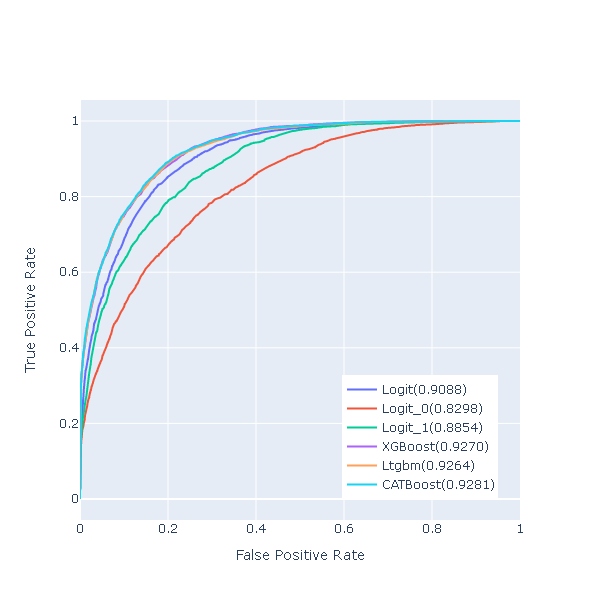
\includegraphics[width=5.0in]{images/newplot.png}
		\caption{}
		\label{WE}
	\end{center}
\end{figure}




最后利用test.csv的数据进行预测,代码如下。
    \begin{tcolorbox}[breakable, size=fbox, boxrule=1pt, pad at break*=1mm,colback=cellbackground, colframe=cellborder]
	\prompt{In}{incolor}{ }{\boxspacing}
	\begin{Verbatim}[commandchars=\\\{\}]
\PY{n}{predictY} \PY{o}{=} \PY{n}{pd}\PY{o}{.}\PY{n}{DataFrame}\PY{p}{(}\PY{n}{XGBoost}\PY{o}{.}\PY{n}{model\PYZus{}fitted}\PY{o}{.}\PY{n}{predict\PYZus{}proba}\PY{p}{(}\PY{n}{nonlinear\PYZus{}sndf\PYZus{}test}\PY{o}{.}\PY{n}{iloc}\PY{p}{[}\PY{p}{:}\PY{p}{,}\PY{l+m+mi}{1}\PY{p}{:}\PY{p}{]}\PY{p}{)}\PY{p}{[}\PY{p}{:}\PY{p}{,}\PY{l+m+mi}{1}\PY{p}{]}\PY{p}{)}
\PY{n}{predictY}\PY{o}{.}\PY{n}{to\PYZus{}csv}\PY{p}{(}\PY{l+s+s1}{\PYZsq{}}\PY{l+s+s1}{Results\PYZus{}1.csv}\PY{l+s+s1}{\PYZsq{}}\PY{p}{,} \PY{n}{encoding} \PY{o}{=} \PY{l+s+s1}{\PYZsq{}}\PY{l+s+s1}{utf\PYZhy{}8}\PY{l+s+s1}{\PYZsq{}}\PY{p}{,} \PY{n}{index}\PY{o}{=}\PY{k+kc}{False} \PY{p}{,} \PY{n}{header}\PY{o}{=}\PY{k+kc}{False}\PY{p}{)}
\PY{n}{predictY2} \PY{o}{=} \PY{n}{pd}\PY{o}{.}\PY{n}{DataFrame}\PY{p}{(}\PY{n}{Ltgbm}\PY{o}{.}\PY{n}{model\PYZus{}fitted}\PY{o}{.}\PY{n}{predict\PYZus{}proba}\PY{p}{(}\PY{n}{nonlinear\PYZus{}sndf\PYZus{}test}\PY{o}{.}\PY{n}{iloc}\PY{p}{[}\PY{p}{:}\PY{p}{,}\PY{l+m+mi}{1}\PY{p}{:}\PY{p}{]}\PY{p}{)}\PY{p}{[}\PY{p}{:}\PY{p}{,}\PY{l+m+mi}{1}\PY{p}{]}\PY{p}{)}
\PY{n}{predictY2}\PY{o}{.}\PY{n}{to\PYZus{}csv}\PY{p}{(}\PY{l+s+s1}{\PYZsq{}}\PY{l+s+s1}{Results\PYZus{}2.csv}\PY{l+s+s1}{\PYZsq{}}\PY{p}{,} \PY{n}{encoding} \PY{o}{=} \PY{l+s+s1}{\PYZsq{}}\PY{l+s+s1}{utf\PYZhy{}8}\PY{l+s+s1}{\PYZsq{}}\PY{p}{,} \PY{n}{index}\PY{o}{=}\PY{k+kc}{False} \PY{p}{,} \PY{n}{header}\PY{o}{=}\PY{k+kc}{False}\PY{p}{)}
\PY{n}{predictY3} \PY{o}{=} \PY{n}{pd}\PY{o}{.}\PY{n}{DataFrame}\PY{p}{(}\PY{n}{CATBoost}\PY{o}{.}\PY{n}{model\PYZus{}fitted}\PY{o}{.}\PY{n}{predict\PYZus{}proba}\PY{p}{(}\PY{n}{nonlinear\PYZus{}sndf\PYZus{}test}\PY{o}{.}\PY{n}{iloc}\PY{p}{[}\PY{p}{:}\PY{p}{,}\PY{l+m+mi}{1}\PY{p}{:}\PY{p}{]}\PY{p}{)}\PY{p}{[}\PY{p}{:}\PY{p}{,}\PY{l+m+mi}{1}\PY{p}{]}\PY{p}{)}
\PY{n}{predictY3}\PY{o}{.}\PY{n}{to\PYZus{}csv}\PY{p}{(}\PY{l+s+s1}{\PYZsq{}}\PY{l+s+s1}{Results\PYZus{}3.csv}\PY{l+s+s1}{\PYZsq{}}\PY{p}{,} \PY{n}{encoding} \PY{o}{=} \PY{l+s+s1}{\PYZsq{}}\PY{l+s+s1}{utf\PYZhy{}8}\PY{l+s+s1}{\PYZsq{}}\PY{p}{,} \PY{n}{index}\PY{o}{=}\PY{k+kc}{False} \PY{p}{,} \PY{n}{header}\PY{o}{=}\PY{k+kc}{False}\PY{p}{)}
	\end{Verbatim}
\end{tcolorbox}

\newpage
\bibliographystyle{abbrv}
\bibliography{biblio}
\end{document}
